\documentclass[preprint]{elsarticle}
% vi:spell spelllang=en

\usepackage{hyperref}

\usepackage[english]{babel}
\usepackage[utf8]{inputenc}
\usepackage[T1]{fontenc}

\usepackage{amsmath}  % Maths
\usepackage{amsfonts} % Maths
\usepackage{amssymb}  % Maths
\usepackage{stmaryrd} % Maths (crochets doubles)

\usepackage{url}     % Mise en forme + liens pour URLs
\usepackage{array}   % Tableaux évolués

\usepackage{comment}


\usepackage{prettyref}
\newrefformat{def}{Def.~\ref{#1}}
\newrefformat{fig}{Fig.~\ref{#1}}
\newrefformat{pro}{Property~\ref{#1}}
\newrefformat{pps}{Proposition~\ref{#1}}
\newrefformat{lem}{Lemma~\ref{#1}}
\newrefformat{thm}{Theorem~\ref{#1}}
\newrefformat{sec}{Sect.~\ref{#1}}
\newrefformat{ssec}{Subsect.~\ref{#1}}
\newrefformat{sssec}{Subsect.~\ref{#1}}
\newrefformat{suppl}{Appendix~\ref{#1}}
\newrefformat{eq}{Eq.~\eqref{#1}}
\newrefformat{ex}{Example~\ref{#1}}
\newrefformat{tb}{Table~\ref{#1}}
\def\pref{\prettyref}

\newdefinition{definition}{Definition}
\newdefinition{property}{Property}
\newdefinition{proposition}{Proposition}
\newdefinition{example}{Example}

\usepackage{tikz}
\newdimen\pgfex
\newdimen\pgfem
\usetikzlibrary{arrows,shapes,shadows,scopes}
\usetikzlibrary{positioning}
\usetikzlibrary{matrix}
\usetikzlibrary{decorations.text}
\usetikzlibrary{decorations.pathmorphing}

% Macros relatives à la traduction de PH avec arcs neutralisants vers PH à k-priorités fixes

% Macros générales
\def\Pint{\textsc{PINT}}

% Notations générales pour PH
\newcommand{\PH}{\mathcal{PH}}
\newcommand{\PHs}{\Sigma}
\newcommand{\PHl}{L}
%\newcommand{\PHp}{\mathcal{P}}
\newcommand{\PHp}{\textcolor{red}{\mathcal{P}}}
\newcommand{\PHproc}{\mathcal{P}}
\newcommand{\PHa}{\PHh}
\newcommand{\PHh}{\mathcal{H}}
\newcommand{\PHn}{\mathcal{N}}

\newcommand{\PHhitter}{\mathsf{hitter}}
\newcommand{\PHtarget}{\mathsf{target}}
\newcommand{\PHbounce}{\mathsf{bounce}}
\newcommand{\PHsort}{\Sigma}

\def\f#1{\mathsf{#1}}
\def\focals{\f{focals}}
\def\play{\cdot}
\def\configs#1{\mathbb C_{#1\rightarrow a}}

%\newcommand{\PHfrappeR}{\textcolor{red}{\rightarrow}}
%\newcommand{\PHmonte}{\textcolor{red}{\Rsh}}

\newcommand{\PHfrappeA}{\rightarrow}
\newcommand{\PHfrappeB}{\Rsh}
%\newcommand{\PHfrappe}[3]{\mbox{$#1\PHfrappeA#2\PHfrappeB#3$}}
%\newcommand{\PHfrappebond}[2]{\mbox{$#1\PHfrappeB#2$}}
\newcommand{\PHfrappe}[3]{#1\PHfrappeA#2\PHfrappeB#3}
\newcommand{\PHfrappebond}[2]{#1\PHfrappeB#2}
\newcommand{\PHobjectif}[2]{\mbox{$#1\PHfrappeB^*\!#2$}}
\newcommand{\PHconcat}{::}
\newcommand{\PHneutralise}{\rtimes}

\def\PHget#1#2{{#1[#2]}}
%\newcommand{\PHchange}[2]{#1\langle #2 \rangle}
\newcommand{\PHchange}[2]{(#1 \Lleftarrow #2)}
\newcommand{\PHarcn}[2]{\mbox{$#1\PHneutralise#2$}}
\newcommand{\PHjoue}{\cdot}

\newcommand{\PHetat}[1]{\mbox{$\langle #1 \rangle$}}


% Notations spécifiques à ce papier
\newcommand{\PHdirectpredec}[1]{\PHs^{-1}(#1)}
\newcommand{\PHpredec}[1]{\f{pred}(#1)}
\newcommand{\PHpredecgene}[1]{\f{reg}({#1})}
\newcommand{\reg}{\PHpredecgene}
\newcommand{\PHpredeccs}[1]{\PHpredec{#1} \setminus \Gamma}

\newcommand{\PHincl}[2]{#1 :: #2}

\def\ctx{\varsigma}
\def\ctxOverride{\Cap}
\def\state#1{\langle #1 \rangle}

% Notations spécifiques aux graphes d'états
%\newcommand{\PHge}{\textcolor{red}{\mathcal{GE}}}
%\newcommand{\PHt}{\mathcal{T}}
%\newcommand{\GE}{\mathcal{GE}}
%\newcommand{\GEt}{\mathcal{T}}
%\newcommand{\GEl}{\PHl}
%\newcommand{\GEa}{\PHa}
%\newcommand{\GEva}[3]{#1 \stackrel{#2}{\longrightarrow} #3}
%\newcommand{\GEval}[3]{#1 \stackrel{#2}{\Longrightarrow} #3}
%\newcommand{\GEget}[2]{\PHget{#1}{#2}}


\def\DEF{\stackrel{\Delta}=}
\def\EQDEF{\stackrel{\Delta}\Leftrightarrow}
\def\SUBSETDEF{\stackrel{\Delta}\subset}

\newcommand{\segmllabel}{\llbracket}
\newcommand{\segmrlabel}{\rrbracket}
\newcommand{\segm}[2]{\segmllabel #1 ; #2 \segmrlabel}
\newcommand{\leqsegm}{\leq_{\segmllabel\segmrlabel}}
\newcommand{\ltsegm}{<_{\llbracket\rrbracket}}

\newcommand{\irB}{B}
\newcommand{\irF}{F}

\usepackage{ifthen}
\usepackage{tikz}
\usetikzlibrary{arrows,shapes}

\definecolor{lightgray}{rgb}{0.8,0.8,0.8}
\definecolor{lightgrey}{rgb}{0.8,0.8,0.8}

\tikzstyle{boxed ph}=[]
\tikzstyle{sort}=[fill=lightgray,rounded corners]
\tikzstyle{process}=[circle,draw,minimum size=15pt,fill=white,
font=\footnotesize,inner sep=1pt]
\tikzstyle{black process}=[process, fill=black,text=white, font=\bfseries]
\tikzstyle{gray process}=[process, draw=black, fill=lightgray]
\tikzstyle{current process}=[process, draw=black, fill=lightgray]
\tikzstyle{process box}=[white,draw=black,rounded corners]
\tikzstyle{tick label}=[font=\footnotesize]
\tikzstyle{tick}=[black,-]%,densely dotted]
\tikzstyle{hit}=[->,>=angle 45]
\tikzstyle{selfhit}=[min distance=30pt,curve to]
\tikzstyle{bounce}=[densely dotted,->,>=latex]
\tikzstyle{hl}=[font=\bfseries,very thick]
\tikzstyle{hl2}=[hl]
\tikzstyle{nohl}=[font=\normalfont,thin]

\newcommand{\currentScope}{}
\newcommand{\currentSort}{}
\newcommand{\currentSortLabel}{}
\newcommand{\currentAlign}{}
\newcommand{\currentSize}{}

\newcounter{la}
\newcommand{\TSetSortLabel}[2]{
  \expandafter\repcommand\expandafter{\csname TUserSort@#1\endcsname}{#2}
}
\newcommand{\TSort}[4]{
  \renewcommand{\currentScope}{#1}
  \renewcommand{\currentSort}{#2}
  \renewcommand{\currentSize}{#3}
  \renewcommand{\currentAlign}{#4}
  \ifcsname TUserSort@\currentSort\endcsname
    \renewcommand{\currentSortLabel}{\csname TUserSort@\currentSort\endcsname}
  \else
    \renewcommand{\currentSortLabel}{\currentSort}
  \fi
  \begin{scope}[shift={\currentScope}]
  \ifthenelse{\equal{\currentAlign}{l}}{
    \filldraw[process box] (-0.5,-0.5) rectangle (0.5,\currentSize-0.5);
    \node[sort] at (-0.2,\currentSize-0.4) {\currentSortLabel};
   }{\ifthenelse{\equal{\currentAlign}{r}}{
     \filldraw[process box] (-0.5,-0.5) rectangle (0.5,\currentSize-0.5);
     \node[sort] at (0.2,\currentSize-0.4) {\currentSortLabel};
   }{
    \filldraw[process box] (-0.5,-0.5) rectangle (\currentSize-0.5,0.5);
    \ifthenelse{\equal{\currentAlign}{t}}{
      \node[sort,anchor=east] at (-0.3,0.2) {\currentSortLabel};
    }{
      \node[sort] at (-0.6,-0.2) {\currentSortLabel};
    }
   }}
  \setcounter{la}{\currentSize}
  \addtocounter{la}{-1}
  \foreach \i in {0,...,\value{la}} {
    \TProc{\i}
  }
  \end{scope}
}

\newcommand{\TTickProc}[2]{ % pos, label
  \ifthenelse{\equal{\currentAlign}{l}}{
    \draw[tick] (-0.6,#1) -- (-0.4,#1);
    \node[tick label, anchor=east,text width=.2cm,align=right] at (-0.55,#1) {#2};
   }{\ifthenelse{\equal{\currentAlign}{r}}{
    \draw[tick] (0.6,#1) -- (0.4,#1);
    \node[tick label, anchor=west,text width=.2cm,align=left] at (0.55,#1) {#2};
   }{
    \ifthenelse{\equal{\currentAlign}{t}}{
      \draw[tick] (#1,0.6) -- (#1,0.4);
      \node[tick label, anchor=south] at (#1,0.55) {#2};
    }{
      \draw[tick] (#1,-0.6) -- (#1,-0.4);
      \node[tick label, anchor=north] at (#1,-0.55) {#2};
    }
   }}
}
\newcommand{\TSetTick}[3]{
  \expandafter\repcommand\expandafter{\csname TUserTick@#1_#2\endcsname}{#3}
}

\newcommand{\myProc}[3]{
  \ifcsname TUserTick@\currentSort_#1\endcsname
    \TTickProc{#1}{\csname TUserTick@\currentSort_#1\endcsname}
  \else
    \TTickProc{#1}{#1}
  \fi
  \ifthenelse{\equal{\currentAlign}{l}\or\equal{\currentAlign}{r}}{
    \node[#2] (\currentSort_#1) at (0,#1) {#3};
  }{
    \node[#2] (\currentSort_#1) at (#1,0) {#3};
  }
}
\newcommand{\TSetProcStyle}[2]{
  \expandafter\repcommand\expandafter{\csname TUserProcStyle@#1\endcsname}{#2}
}
\newcommand{\TProc}[1]{
  \ifcsname TUserProcStyle@\currentSort_#1\endcsname
    \myProc{#1}{\csname TUserProcStyle@\currentSort_#1\endcsname}{}
  \else
    \myProc{#1}{process}{}
  \fi
}

\newcommand{\repcommand}[2]{
  \providecommand{#1}{#2}
  \renewcommand{#1}{#2}
}
\newcommand{\THit}[5]{
  \path[hit] (#1) edge[#2] (#3#4);
  \expandafter\repcommand\expandafter{\csname TBounce@#3@#5\endcsname}{#4}
}
\newcommand{\TBounce}[4]{
  (#1\csname TBounce@#1@#3\endcsname) edge[#2] (#3#4)
}

\newcommand{\TState}[1]{
  \foreach \proc in {#1} {
    \node[current process] (\proc) at (\proc.center) {};
  }
}

% Macros spécifiques au Modèle de Thomas / aux RRB

\newcommand{\sN}{\mathbb{N}}

% Notations pour le modèle de Thomas (depuis thèse)
\newcommand{\GRN}{\mathcal{GRN}}
\newcommand{\IG}{\mathcal{G}}
%\def\IG{\mathrm{IG}}
\newcommand{\GRNreg}[1]{E^{-1}(#1)}
\newcommand{\GRNreslabel}{\mathsf{Res}}
\newcommand{\GRNres}[2]{\GRNreslabel_{#1}(#2)}
%\newcommand{\GRNallres}[1]{\mathsf{Res}_{#1}}
\newcommand{\GRNallres}[1]{\textcolor{red}{\mathsf{Res}_{#1}}}
\newcommand{\GRNget}[2]{\PHget{#1}{#2}}
\newcommand{\GRNstate}[1]{\PHetat{#1}}
\newcommand{\GRNstates}{\mathcal{S}}
\newcommand{\GRNedgef}[4]{#1 \xrightarrow{#2 #3} #4}
\newcommand{\GRNedge}[4]{\GRNedgef{#1}{#2,}{#3}{#4}}
\newcommand{\GRNtrans}[2]{#1 \rightarrow #2}
\newcommand{\uns}{\pm}

\def\levelsl{\mathsf{levels}}
\def\levels#1#2{\levelsl(#1\rightarrow #2)}
\def\ulevels#1#2{\overline{\levelsl}(#1\rightarrow #2)}
%\def\levelsA#1#2{\levels_+(#1\rightarrow #2)}
%\def\levelsI#1#2{\levels_-(#1\rightarrow #2)}
\def\levelsA#1#2{\textcolor{red}{\levelsl_+(#1\rightarrow #2)}}
\def\levelsI#1#2{\textcolor{red}{\levelsl_-(#1\rightarrow #2)}}
%\newcommand{\PHres}{\mathsf{Res}}

\newcommand{\Kinconnu}{\emptyset}
\newcommand{\RRGva}[3]{#1 \stackrel{#2}{\longrightarrow} #3}
\newcommand{\RRGgi}{\mathcal{G}}
\newcommand{\RRGreg}[1]{\RRGgi_{#1}}



%\definecolor{darkred}{rgb}{0.5,0,0}
%\definecolor{lightred}{rgb}{1,0.8,0.8}
%\definecolor{lightgreen}{rgb}{0.7,1,0.7}
\definecolor{darkgreen}{rgb}{0,0.5,0}
%\definecolor{darkyellow}{rgb}{0.5,0.5,0}
%\definecolor{lightyellow}{rgb}{1,1,0.6}
%\definecolor{darkcyan}{rgb}{0,0.6,0.6}
%\definecolor{darkorange}{rgb}{0.8,0.2,0}

%\definecolor{notsodarkgreen}{rgb}{0,0.7,0}

%\definecolor{coloract}{rgb}{0,1,0}
%\definecolor{colorinh}{rgb}{1,0,0}
\colorlet{coloract}{darkgreen}
\colorlet{colorinh}{red}
%\colorlet{coloractgray}{lightgreen}
%\colorlet{colorinhgray}{lightred}
%\colorlet{colorinf}{darkgray}
%\colorlet{coloractgray}{lightgreen}
%\colorlet{colorinhgray}{lightred}

%\colorlet{colorgray}{lightgray}


\tikzstyle{grn}=[every node/.style={circle,draw=black,outer sep=2pt,minimum
                size=15pt,text=black}, node distance=1.5cm]
\tikzstyle{act}=[->,draw=black,thick,color=black]
\tikzstyle{inh}=[>=|,-|,draw=black,thick, text=black,label]
%\tikzstyle{inh}=[>=|,-|,draw=colorinh,thick, text=black,label]
%\tikzstyle{act}=[->,>=triangle 60,draw=coloract,thick,color=coloract]
%\tikzstyle{inhgray}=[>=|,-|,draw=colorinhgray,thick, text=black,label]
%\tikzstyle{actgray}=[->,>=triangle 60,draw=coloractgray,thick,color=coloractgray]
\tikzstyle{inf}=[->,draw=colorinf,thick,color=colorinf]
%\tikzstyle{elabel}=[fill=none, above=-1pt, sloped,text=black, minimum size=10pt, outer sep=0, font=\scriptsize,draw=none]
\tikzstyle{elabel}=[fill=none,text=black, above=-2pt,%sloped,
minimum size=10pt, outer sep=0, font=\scriptsize, draw=none]
%\tikzstyle{elabel}=[]
\tikzstyle{sg}=[every node/.style={outer sep=2pt,minimum
                size=15pt,text=black}, node distance=2cm]



% Commandes À FAIRE
\usepackage{color} % Couleurs du texte
\newcommand{\todo}[1]{\textcolor{red}{\textbf{[TODO: #1]}}}
%\newcommand{\rewrite}[1]{\rewriteil{REWRITE: #1}}


\def\modMF#1{\textcolor{teal}{#1}}
\def\modLP#1{\textcolor{magenta}{#1}}
\def\modMM#1{\textcolor{blue}{#1}}
\def\modOR#1{\textcolor{olive}{#1}}



% Id est
\newcommand{\ie}{i.e.~}

% Césures
\hyphenation{pa-ra-me-tri-za-tion}
\hyphenation{pa-ra-me-tri-za-tions}



\begin{document}

\begin{frontmatter}

\title{\modLP{Identification of} Biological Regulatory Networks from Process Hitting models}
%\\\rewriteil{Or possibly: “Complementarity between PH, IG and Thomas modeling”}

\author[irccyn,nii]{Maxime Folschette}
\ead{Maxime.Folschette@irccyn.ec-nantes.fr}
\author[lri]{Lo\"ic Paulev\'e}
\author[nii]{Katsumi Inoue}
\author[irccyn,nii]{Morgan Magnin}
\author[irccyn]{Olivier Roux}

\address[irccyn]{LUNAM Universit\'e, \'Ecole Centrale de Nantes, IRCCyN UMR CNRS 6597\\
(Institut de Recherche en Communications et Cybern\'etique de Nantes)\\
1 rue de la No\"e - B.P. 92101 - 44321 Nantes Cedex 3, France.}
\address[nii]{National Institute of Informatics,\\
2-1-2, Hitotsubashi, Chiyoda-ku, Tokyo 101-8430, Japan.}
\address[lri]{CNRS, Laboratoire de Recherche en Informatique UMR CNRS 8623\\
Universit\'e Paris-Sud, 91405 Orsay Cedex, France}


\begin{abstract}
\modMF{Maxime}
\modLP{Lo\"ic}
\modMM{Morgan}
\modOR{Olivier}

%\parindent 0.5cm
The Process Hitting (PH) \modLP{is a particular class of Indeterministic Asynchronous Automata
Network (or safe Petri nets) on which have been recently designed several static analyses for
dynamical properties that are tractable on very large systems.}

\modLP{In this paper, we address the formal identification of qualitative
models of Biological Regulatory Networks (BRNs) from PH models.}
First, the inference of the Interaction Graph (IG) from a PH model
\modLP{summarizes the signed influences between the components} that are effective for the dynamics.
Second, we provide the inference of all Ren\'e Thomas models of BRNs 
that are compatible with a given PH.
As the PH allows the specification of indeterministic interactions between
components, our inference emphasizes the ability of PH to deal with large BRNs with incomplete knowledge
on interactions, where Thomas' approach fails because of the combinatorics of parameters.

The inference of corresponding Thomas models is provided using Answer Set Programming,
which allows notably an efficient enumeration of (possibly numerous) compatible parametrizations.

%\todo{Rather name Kaufman as the creator of BRNs.}
%On the other hand, the qualitative modeling of BRNs has been widely addressed using Ren\'e Thomas'
%formalism, leading to numerous theoretical work and practical tools to understand emerging behaviors.
%In addition to be able to use the existing results on this formalism,
%obtaining the Thomas representation of a PH model allows to iteratively refine a model.
%Linking this representation to PH would not only allow to use the existing results on this formalism,
%but also to iteratively refine the model of a system.

%This paper establishes formal links between these two formalisms, permitting to appreciate their
%complementary features.
\end{abstract}

\begin{keyword}
qualitative modeling \sep
model abstraction \sep
interaction graph \sep
René Thomas' parameters \sep
answer set programming
\end{keyword}

\end{frontmatter}



% vim:spell spelllang=en:
\section{Introduction}\label{sec:intro}

As regulatory phenomena play a crucial role in biological systems, they need to be studied accurately.
Biological Regulatory Networks (BRNs) consist in sets of either positive or negative mutual effects between the components.
With the purpose of analyzing these systems, they are often modeled as graphs which make it possible to determine the possible evolutions of all the interacting components of the system.
\modOR{Besides continuous models of physicists, generally designed through systems of ordinary differential equations, modeling regulatory networks by means of Boolean networks has become popular in the wake of Kauffman work \cite{kauffman1969metabolic}.
We based our work on a logical formalism developed by Ren\'e Thomas from 1973 \cite{Thomas73} that generalizes upon Boolean networks in the sense that it allows variables to have more than two values and transitions between states to occur asynchronously.}

In this approach, the different levels of a component, such as concentration or expression levels, are abstractly represented by (positive) integer values and transitions between these levels may be considered as instantaneous.
Hence, qualitative state graphs may be derived from which we are able to formally find out all the possible behaviors expressed as sequences of transitions between these states.
Nevertheless, these dynamics can be precisely established only with regard to some discrete parameters,
hereafter called ``Thomas' parameters'',
which stand for kinds of ``focal points'', \ie the evolutionary tendency from each state and depending on the set of the other currently interacting components.
%resources in this very state, that is, the set of the other currently interacting components.
%Hereafter, we refer to these discrete parameters as Thomas' parameters.

Thomas' modeling has motivated numerous works around the link between the Interaction Graph (IG)
(summarizing the global influences between components) and the possible dynamics (e.g.,
\cite{RiCo07,RRT08}),
model reduction (e.g., \cite{Naldi09}), formal checking of dynamics (e.g., \cite{Richard06,Naldi07}), 
and the incorporation of time (e.g., \cite{Siebert06,Ahmad08}) and probability
(e.g., \cite{Twardziok10-CMSB}) dimensions, to name but a few.

While the formal checking of dynamical properties is often limited to small networks because of the
state graph explosion, an other major drawback of this framework is the difficulty to
specify Thomas' parameters, especially for large networks. \modOR{Other works have also been carried out with the aim of dealing with large systems (e.g. \cite{Corblin200991,Bollman2007,Delaplace2012, 10.1371/journal.pone.0007992}).} \modMM{Because of the complexity of such systems, these works generaly focus on some restricted properties,} \modOR{as finding out steady states.} 
%\todo{The reviewer proposes to nuance this with several papers:
%\begin{itemize}
%  \item Corblin, F., Tripodi, S., Fanchon, E., Ropers, D., \& Trilling, L. (2009).
%    A declarative constraint-based method for analyzing discrete genetic
%    regulatory networks. Bio Systems, 98(2), 91104.
%  \item Bollman, D., Coln-Reyes, O., \& Orozco, E. (2007). Fixed points in
%    discrete models for regulatory genetic networks. EURASIP journal on
%    bioinformatics \& systems biology, 2007, 97356.
%  \item Delaplace, F., Klaudel, H., Melliti, T., \& Sen, S. (2012). Analysis
%    of modular organisation of interaction networks based on asymptotic
%    dynamics. In D. Gilbert \& M. Heiner (Eds.), CMSB 2012
%  \item Scalable Steady State Analysis of Boolean Biological Regulatory Net-
%    works Ay F, Xu F, Kahveci T (2009) Scalable Steady State Analysis
%    of Boolean Biological Regulatory Networks. PLoS ONE 4(12): e7992.
%\end{itemize}
%This can be in turn be nuanced as some papers only focus on rather specific aspects (like steady-states for instance).}

In order to address the formal analysis of additional dynamical properties \modMM{(e.g., state reachabilities)} within very large BRNs, we recently
introduced in \cite{PMR10-TCSB} a new formalism, named the \emph{Process Hitting} (PH), to model
concurrent systems having components with a few qualitative levels.
A PH model describes, in an atomic manner, the possible evolutions of a process (representing one
component at one level) triggered by the hit of at most one other process in the system.
This framework can be seen as a special class of formalisms like Petri Nets or Communicating Finite
State Machines, where the arity and the effect of synchronizations between components are
restricted.
Thanks to the particular structure of interactions within a PH, very efficient static analysis
methods have been developed to over- and under-approximate reachability properties making tractable
the formal analysis of the qualitative dynamics of BRNs with hundreds or thousands of components,
which was impossible with other state-of-the-art approaches \cite{PMR12-MSCS,PAK13-CAV,FPMR13-CS2Bio}.
 
The PH is suitable to model BRNs with different levels of abstraction in the specification of
cooperations (associated influences) between components. \modOR{The concept of cooperation refers to the} \modMM{way two (or more) components jointly influence a third one. In other words, it captures the logical functions stating how} \modOR{various elements coalesce and act together upon an other element among the network.}
\modLP{In particular, PH allows to specify partial (non-deterministic) cooperations that superpose the dynamics of 
candidate fully-specified (deterministic) cooperations.
This permit to model BRNs with a partial knowledge on precise evolution functions for components
by capturing the largest (the most general) dynamics, without a combinatorics enumeration of
compatible Thomas models.}

\medskip

The aim of this paper is to formally establish links between several layers suited for specifying the
qualitative dynamics of BRNs, namely:
the Interaction Graph (IG), referencing the sign of direct regulations between components;
the Process Hitting (PH), which permits to specify the qualitative dynamics of the system with
various degrees of knowledge for joint regulations;
and Thomas' parameters, which completely specify the functions governing the evolution of
components.
Another motivation for the work depicted in this paper is that it constitutes an important step
to go further in the study of large biological regulatory networks systems beyond simple analysis:
it makes it possible to partly control some behaviors.
Indeed, when one wants to modify some behaviors
(e.g.~so as to avoid the reachability of some states or to create stable states)
we intend to be able to get upstream the results in accordance at the regulatory level.
The outcome of the present work is that we could make such changes on the PH model
and then recover afterwards the BRN corresponding to the transformed behavioral system.
In a more general framework and in an interesting way,
we should be able to synthesize families of BRN having some featuring behavioral properties.

Firstly, we derive rules that, given a PH model, infer the IG corresponding to the dynamics of the
encoded BRN.
The obtained IG relates only components that have actual influence in the dynamics.
This typically results into IGs that contain less interactions than an hypothetical starting prior
IG, as the specification of component evolutions may reveal non-functional regulations.
Based on the derived IG, various static analysis allows to conclude on global properties
of the system dynamics (see \cite{PR11-SASB} for a short survey).
The most known are the Thomas' conjectures (that have been proved since,
e.g.~\cite{RRT08,RiCo07,Richard2010378}
for Boolean and discrete networks),
which relate the absence of
positive cycle to the impossibility for multi-stationarity (distinct attractors),
and the absence of negative cycle to the impossibility for oscillatory behaviors.

Second, we tackle the inference of Thomas' parameters that are compatible with a given PH
model, \ie that fully specify the evolution of components while respecting the cooperations
specified in PH.
More formally, the resulting BRN dynamics is ensured to be included in the PH dynamics: any
transition in the (asynchronous) Thomas model exists in the PH model.
In practice, the number of compatible Thomas parameters can be huge for large networks where only a
few cooperations are specified.
This highlights that the PH is suitable to analyze dynamics of large-scale networks
where the knowledge on cooperations is often incomplete:
instead of dealing with a possibly non-tractable number of Thomas models, one can already capture
precise dynamical features using a single PH model which gathers all the plausible dynamics.

Finally, we discuss on an implementation of these inference schemes using Answer Set
Programming (ASP) \cite{Baral03},  which turns out to be effective for these enumerative searches.
The whole method is also applied to the biological model of ERBB receptor-regulated G1/S transition,
containing 20 components,
which allows to detail how joint actions can be defined inside a PH model in order
to refine its dynamics, and study a more precise class of underlying Thomas models.
%\todo{describe application}

Our work is related to the approach of \cite{Khalis09} which relies on temporal logic, and \cite{20646302,DBLP:conf/ipcat/CorblinFTCT12} which also uses constraint programming.
Both aim at determining a class of models which are consistent with available partial data on the regulatory structure and dynamical properties.
%These classes are built in order to infer properties common to some studied models.
%In our approach, we intend to focus on the Thomas' parameters inference
Our method is based on a model rather than on constraints, which allows to define some properties on the system structure (such as cooperations).
Furthermore, we claim that we are able to deal with larger biological networks.
Finally, it must be noticed that we are not interested in this paper in the derivation of one PH
from a BRN (which was previously described in \cite{PMR10-TCSB}) but, on the contrary, in finding
out a set of BRNs from one PH.

The contributions presented in this paper significantly extend and improve the preliminary results
introduced in \cite{FPIMR12-CMSB}.
In addition to the improvement of the efficiency and accuracy of the IG inference, we have added support for
\modLP{non-monotonous} regulations, that are regulations being positive or negative depending on a particular
context.
This allows to apply our methodology to a wider class of models.
Furthermore, some parts have been completely rewritten in order to explain more precisely the efficiency of the ASP implementation,
and give a new detailed biological application of our work.

\paragraph{Outline}
\pref{sec:frameworks} recalls the PH and Thomas frameworks;
\pref{sec:infer-IG} defines the IG inference from PH;
\pref{sec:infer-K} details the parameters inference and the enumeration of Thomas parametrizations compatible with a PH;
\pref{sec:impl} discusses the implementation of the latter in ASP.
\pref{sec:examples} illustrates our method on a biological model
and discusses its applicability on large models.

\paragraph{Notations}
$\segm{i}{j}$ is the set of integers $\{ i, i+1, \dots, j \}$.


\section{Frameworks}\label{sec:frameworks}
\subsection{The Process Hitting framework}
\label{ssec:PH}

We recall here the definition and semantics of the Process Hitting (PH), and its usage to model
cooperation between concurrent components.
Two examples of PH modeling a BRN at different abstraction levels are given.
They serve as running examples in the rest of this article.

\medskip

A PH (\pref{def:PH}) gathers a finite number of concurrent \emph{processes}
grouped into a finite set of \emph{sorts}.
A process belongs to a unique sort and is noted $a_i$ where $a$ is the
sort and $i$ the identifier of the process within the sort $a$.
At any time, one and only one process of each sort is present; a state of the PH thus corresponds to the set of such processes.
 
The concurrent interactions between processes are defined by a set of
\emph{actions}.
Actions describe the replacement of a process by another of the same sort
conditioned by the presence of at most one other process in the current
state of the PH.
An action is denoted by $\PHfrappe{a_i}{b_j}{b_k}$ where $a_i,b_j,b_k$ are processes
of sorts $a$ and $b$.
It is required that $b_j\neq b_k$ and that $a=b\Rightarrow a_i=b_j$.
An action $h=\PHfrappe{a_i}{b_j}{b_k}$ is read as ``$a_i$ \emph{hits} $b_j$ to
make it bounce to $b_k$'', and
$a_i,b_j,b_k$ are called respectively \emph{hitter}, \emph{target} and
\emph{bounce} of the action, and can be referred to as
$\PHhitter(h), \PHtarget(h), \PHbounce(h)$, respectively.

\begin{definition}[Process Hitting]\label{def:PH}
A \emph{Process Hitting} is a triple $(\PHs,\PHl,\PHa)$:
\begin{itemize}
\item $\PHs \DEF \{a,b,\dots\}$ is the finite set of \emph{sorts};
\item $\PHl \DEF \prod_{a\in\PHs} \PHl_a$ is the set of states with $\PHl_a = \{a_0,\dots,a_{l_a}\}$
the finite set of \emph{processes} of sort $a\in\Sigma$ and $l_a$ a positive integer with
	$a\neq b\Rightarrow \forall(a_i,b_j)\in\PHl_a\times\PHl_b,a_i\neq b_j$;
\item $\PHa \DEF \{ \PHfrappe{a_i}{b_j}{b_k}, \ldots \mid
					(a,b)\in\PHs^2 \wedge (a_i,b_j,b_k)\in \PHl_a\times\PHl_b\times\PHl_b$ \\
	\hspace*{2cm} $\wedge b_j\neq b_k \wedge a=b\Rightarrow a_i=b_j\}$
			is the finite set of \emph{actions}.
\end{itemize}
$\PHproc$ denotes the set of all processes ($\PHproc \DEF \{ a_i\mid a\in\PHs \wedge a_i\in\PHl_a\}$).
\end{definition}

\noindent
The sort of a process $a_i$ is referred to as $\PHsort(a_i)=a$ and the set of
sorts present in an action $h\in\PHa$ as 
$\PHsort(h) = \{\PHsort(\PHhitter(h)),\PHsort(\PHtarget(h))\}$.
Given a state $s\in \PHl$, the process of sort $a\in\PHs$ present in $s$ is
denoted by $\PHget{s}{a}$, that is the $a$-coordinate of the state $s$.
If $a_i\in \PHl_a$, we define the notation $a_i\in s \EQDEF \PHget{s}{a}=a_i$.

An action $h=\PHfrappe{a_i}{b_j}{b_k} \in\PHa$ is \emph{playable} in $s\in L$
if and only if $\PHget{s}{a}=a_i$ and $\PHget{s}{b}=b_j$.
In such a case, $(s\play h)$ stands for the state resulting from the play of
the action $h$ in $s$, that is 
$\PHget{(s\play h)}{b} = b_k$ and 
$\forall c\in\PHs, c\neq b, \PHget{(s\play h)}{c} = \PHget{s}{c}$.
For the sake of clarity, $((s\play h)\play h')$, $h'\in\PHa$ is abbreviated as
$(s\play h\play h')$.

\begin{example}
\pref{fig:runningPH-1} represents a PH $(\PHs,\PHl,\PHa)$ with
$\PHs = \{a,b,c\}$,
$\PHl_a = \{a_0,a_1,a_2\}$,
$\PHl_b = \{b_0, b_1\}$,
$\PHl_c = \{c_0, c_1\}$, and
\begin{align*}
\PHa & = \{
	\PHfrappe{a_2}{b_1}{b_0},
&&  \PHfrappe{b_0}{a_2}{a_1},
&&	\PHfrappe{c_0}{a_2}{a_1},\\
&&& \PHfrappe{b_0}{a_1}{a_0},
&&	\PHfrappe{c_0}{a_1}{a_0},\\
&&& \PHfrappe{b_1}{a_0}{a_1},
&&	\PHfrappe{c_1}{a_0}{a_1},\\
&&& \PHfrappe{b_1}{a_1}{a_2},
&&	\PHfrappe{c_1}{a_1}{a_2} \}\enspace.
\end{align*}
The action $h=\PHfrappe{b_1}{a_1}{a_2}$ is playable in the state
$s = \state{b_1,a_1,c_0}$; and $s\play h=\state{b_1,a_2,c_0}$.

\begin{figure}[t]
\centering
\scalebox{1.3}{
\begin{tikzpicture}
\TSort{(0,0)}{a}{3}{r}
\TSort{(-3,0.5)}{b}{2}{l}
\TSort{(3,0.5)}{c}{2}{r}

\THit{b_1}{very thick}{a_0}{.west}{a_1}
\THit{b_1}{very thick}{a_1}{.north west}{a_2}
\THit{b_0}{}{a_2}{.west}{a_1}
\THit{b_0}{}{a_1}{.west}{a_0}

\path[bounce, bend left=60]
\TBounce{a_1}{very thick}{a_2}{.south}
\TBounce{a_0}{very thick}{a_1}{.south}
;
\path[bounce, bend right=60]
\TBounce{a_2}{}{a_1}{.north}
\TBounce{a_1}{}{a_0}{.north}
;

\THit{c_1}{very thick}{a_0}{.east}{a_1}
\THit{c_1}{very thick}{a_1}{.north east}{a_2}
\THit{c_0}{}{a_2}{.east}{a_1}
\THit{c_0}{}{a_1}{.east}{a_0}

\path[bounce, bend right=60]
\TBounce{a_1}{very thick}{a_2}{.south east}
\TBounce{a_0}{very thick}{a_1}{.south east}
;
\path[bounce, bend left=60]
\TBounce{a_2}{}{a_1}{.north}
\TBounce{a_1}{}{a_0}{.north east}
;

\THit{a_2}{bend right}{b_1}{.north east}{b_0}
\path[bounce, bend left=80]
\TBounce{b_1}{out=100,in=140}{b_0}{.north}
;

\end{tikzpicture}
}
\caption{\label{fig:runningPH-1}
A Process Hitting (PH) example.
Sorts are represented by labeled boxes, and processes by circles (ticks are
the identifiers of the processes within the sort, for instance, $a_0$ is the
process ticked $0$ in the box $a$).
An action (for instance $\PHfrappe{b_1}{a_1}{a_2}$) is represented by a pair of
directed arcs, having the hit part ($b_1$ to $a_1$) in plain line and the bounce
part ($a_1$ to $a_2$) in dotted line.
Here, actions involving $b_1$ or $c_1$ are in thick lines.
%The current state is represented by the grayed processes:
%$\state{a_0,b_1,c_0,d_0}$.
}
\end{figure}

This PH example actually models a BRN where the component $a$ has three qualitative
levels and components $b$ and $c$ are boolean.
In this BRN, $b$ and $c$ activate $a$, while $a$ inhibits $b$.
The inhibition of $b$ by $a$ is only effective when $a$ is at level $2$ (noted: $a_2$);
in the other cases, $b$ cannot evolve in any direction.
The activation of $a$ by $b$ ($c$) is encoded by the actions making the level of $a$ increase (resp.
decrease) when $b$ ($c$) is present (resp. absent).
It is worth noticing that the activation of $a$ by $b$ ($c$) is independent from $c$ ($b$).
This may express a lack of knowledge on the cooperation between these two regulators:
we thus model an over-approximation of the possible actions.
\end{example}

\paragraph{Modeling cooperation}
As described in \cite{PMR10-TCSB}, the cooperation between several processes to make another process bounce can be
expressed in PH by building a \emph{cooperative sort}.
\pref{fig:PH-cooperativity} shows an example of cooperation between processes $b_1$ and $c_1$ to
make $a_1$ bounce to $a_2$:
a cooperative sort $bc$ is defined with 4 processes (one for each sub-state of the presence of
processes $b_1$ and $c_1$).
For the sake of clarity, the processes of $bc$ are indexed using the sub-state they represent.
Hence, $bc_{01}$ represents the sub-state $\state{b_0,c_1}$, and so on.
Each process of sort $b$ and $c$ hit $bc$ to make it bounce to the process reflecting the status of the sorts $b$
and $c$ (e.g., $\PHfrappe{b_1}{bc_{00}}{bc_{10}}$ and $\PHfrappe{b_1}{bc_{01}}{bc_{11}}$).
Then, it is process $bc_{11}$ which hits $a_1$ to make it bounce to $a_2$ instead of
independent hits from $b_1$ and $c_1$.

\begin{figure}[p]
\centering
\scalebox{1.3}{
\begin{tikzpicture}
\TSort{(0,0)}{b}{2}{t}
\TSort{(0,-3.8)}{c}{2}{b}
\TSort{(4.5,-3)}{a}{3}{r}

\TSetTick{bc}{0}{00}
\TSetTick{bc}{1}{01}
\TSetTick{bc}{2}{10}
\TSetTick{bc}{3}{11}
% \TSetSortLbcel{bc}{$\neg a\wedge b$}
\TSort{(-0.5,-2)}{bc}{4}{b}

\THit{b_1}{very thick,bend right}{bc_0}{.north}{bc_2}
\THit{b_1}{very thick,bend right}{bc_1}{.north}{bc_3}
\THit{b_0}{}{bc_2}{.north west}{bc_0}
\THit{b_0}{}{bc_3}{.north west}{bc_1}

\THit{c_0}{}{bc_1}{.south}{bc_0}
\THit{c_0}{}{bc_3}{.south}{bc_2}
\THit{c_1}{very thick}{bc_0}{.south}{bc_1}
\THit{c_1}{very thick}{bc_2}{.south}{bc_3}

\path[bounce, bend right=25]
\TBounce{bc_2}{}{bc_0}{.north east}
\TBounce{bc_3}{}{bc_1}{.north east}
;
\path[bounce, bend left=80, distance=30]
\TBounce{bc_0}{very thick}{bc_2}{.north}
\TBounce{bc_1}{very thick}{bc_3}{.north}
;
\path[bounce, bend right]
\TBounce{bc_0}{very thick}{bc_1}{.west}
\TBounce{bc_2}{very thick}{bc_3}{.west}
;
\path[bounce, bend left]
\TBounce{bc_3}{}{bc_2}{.east}
\TBounce{bc_1}{}{bc_0}{.east}
;

\THit{bc_3}{}{a_1}{.west}{a_2}
\path[bounce, bend left=40]
\TBounce{a_1}{}{a_2}{.south west}
;

\end{tikzpicture}
}

\caption{\label{fig:PH-cooperativity}
A PH modeling a cooperativity between $b_1$ and $c_1$ to make
$a_1$ bounce to $a_2$.
Actions involving $b_1$ or $c_1$ are in thick lines.
}
\end{figure}
\begin{figure}[p]
\centering
\scalebox{1.3}{
\begin{tikzpicture}
\path[use as bounding box] (-4,-1.9) rectangle (4.5,3.9);

\TSort{(0,0)}{a}{3}{l}
\TSort{(3, 3)}{b}{2}{t}
\TSort{(3,-1)}{c}{2}{b}

\TSetTick{bc}{0}{00}
\TSetTick{bc}{1}{01}
\TSetTick{bc}{2}{10}
\TSetTick{bc}{3}{11}
% \TSetSortLbcel{bc}{$\neg a\wedge b$}
\TSort{(-3,-0.5)}{bc}{4}{l}

\THit{bc_3}{}{a_1}{.north west}{a_2}
\THit{bc_0}{}{a_1}{.south west}{a_0}
\path[bounce]
\TBounce{a_1}{bend left}{a_2}{.south west}
\TBounce{a_1}{bend right}{a_0}{.north west}
;

\THit{b_0}{}{a_2}{.east}{a_1}
\THit{b_1}{}{a_0}{.north east}{a_1}
\path[bounce]
\TBounce{a_2}{bend left}{a_1}{.north east}
\TBounce{a_0}{bend right=20}{a_1}{.south}
;

\THit{c_0}{bend right}{a_2}{.south east}{a_1}
\THit{c_1}{bend right}{a_0}{.east}{a_1}
\path[bounce]
\TBounce{a_2}{bend left=20}{a_1}{.north}
\TBounce{a_0}{bend right=30}{a_1}{.south east}
;

\path[dashed,hit]
	(2,-1.3) edge[bend left=10] (-2.3,-0.7)
	(2.2, 3.3) edge[bend right=10] (-2.3,3)
;

\THit{a_2}{bend left,out=40,in=80}{b_1}{.north west}{b_0}
\path[bounce, bend right]
\TBounce{b_1}{}{b_0}{.east}
;

\end{tikzpicture}
}

\caption{\label{fig:runningPH-2}
PH resulting from the refinement of the one in \pref{fig:runningPH-1} by the
specification of several cooperations.
The actions from $b$ and $c$ to the cooperative sort $bc$ are identical to those defined in
\pref{fig:PH-cooperativity} and are represented here by a single dashed arc.
}
\end{figure}

We note that cooperative sorts are standard PH sorts and do not involve any
special treatment regarding the semantics of related actions.

When the number of cooperating processes is large, it is possible to chain several cooperative sorts
to prevent the combinatoric explosion of the number of processes created within cooperative sorts.
For instance, if $b_1$, $c_1$, and $d_1$ cooperate, one can create a cooperative sort $bc$ with 4
processes reflecting the presence of $b_1$ and $c_1$, and a cooperative sort $bcd$ with 4 processes
reflecting the presence of $bc_{11}$ and $d_1$.  Such constructions are helpful in PH
as the static analysis of dynamics developed in \cite{PMR12-MSCS} does not suffer from the number of
sorts, but on the number of processes within a single sort.

While the construction of cooperation in PH allows to encode any boolean functions
between cooperating processes \cite{PMR10-TCSB}, it is worth noticing they introduce a temporal
shift in their application.
This allows the existence of interleaving of actions leading to a cooperative sort representing a
past sub-state of the presence of the cooperative processes.
The resulting behavior is then an over-approximation
of the realization of an instantaneous cooperation.
However, it is possible to obtain the exact behavior of the cooperations by using the semantics with prioritized actions defined in~\cite{FPMR13-CS2Bio}.
Although this new semantics is not further described here, the inferences given in \pref{sec:infer-IG} \& \ref{sec:infer-K} do ignore the temporal shift induced by the cooperative sorts.

\begin{example}
The PH in \pref{fig:runningPH-2} results from the refinement of the PH in \pref{fig:runningPH-1}
where several cooperations have been specified.
In particular, the bounce to $a_2$ is the result of a cooperation between $b_1$ and $c_1$; and the
bounce to $a_0$ of a cooperation between $b_0$ and $c_0$.
Hence, this PH expresses a BRN where $a$ requires both $b$ and $c$ active to reach its
highest level, and $a$ does not become inactive unless both $b$ and $c$ are inactive.
\end{example}

% vim:spell spelllang=en
\subsection{Thomas's modeling}
\label{ssec:thomas}

%\todo{Name Kaufman as the creator of BRNs.}

\modMM{
The principle of qualitative modeling was introduced as synchronous Boolean networks by Stuart Kauffman on the one hand \cite{kauffman1969metabolic}, and asynchronous Ren\'e-Thomas networks on the other \cite{Thomas73}. Both models have been considered of interest and led to numerous works. In the following, we choose to focus on  Thomas's modeling, with its asynchronous, unitary and multi-level semantics.}

\modMM{In this section, we} concisely present Thomas's modeling of a Biological Regulatory Network (BRN) and its dynamics, merely inspired by
\cite{thomas1990biological, Richard06,BernotSemBRN}.
%In order to enlarge the class of Thomas' models compatible with PH dynamics (w.r.t.~the presented
%inference),
%we propose the notion of unsigned edge modeling an interaction whose nature (activation or inhibition) is undetermined,
%and we extend the classical parametrization formalism by setting parameters to intervals of values instead of single values.
%We briefly discuss these additions.

\medskip

Thomas's formalism lies on two complementary descriptions of the system. First, the
\emph{Interaction Graph} (IG) models the structure of the system by defining the components'
mutual influences and the conditions of these influences. \modMM{
Then t}he \emph{parametrization} \modMM{
removes the ambiguity when a component is targeted by (at least) two different influences. In other words, it} specifies the levels towards which a component tends when a given configuration of its regulators applies.

The IG is composed of nodes ($a$, $b$, $c$, …) that represent components,
and edges ($\GRNedge{a}{s}{t}{b}$, …) labeled with a sign ($s$) and a threshold ($t$) that stand for regulations between these components (\pref{def:ig}).
The activity, concentration rate or presence of each component in a given state of the system is modeled by an abstract discrete value called \emph{expression level}.
The maximum expression level of a component $a$ is denoted $l_a$.
The sign of an edge denotes the kind of regulation it models: it can be positive
($+$), negative ($-$) or \modLP{non-monotonous} ($\uns$),
the latter meaning that \modLP{the regulation have different sign depending on the context \cite{Sene13-TCS}}.
Regarding the dynamics, an edge $\GRNedge{a}{s}{t}{b}$ states that $a$ influences the evolution of $b$ in a certain way when its expression level is above or equal to the threshold $t$;
when its expression level is strictly below this threshold, another kind of influence is expressed, which usually consists of the opposite influence.

\modMM{The IG is not sufficient to unambiguously define the dynamics of the system. In particular, a component may be regulated by both a positive and negative interaction derived from two different components. To refine the dynamics, a parametrization has been added to the model \cite{snoussi1989qualitative}. This parametrization allows to define focal points, \ie it clarifies the level towards which a component evolves depending on the expression of its regulators.
Some of the information included in the IG and the parametrization may appear as slightly redundant. Especially, if the single parametrization were enriched with additional constraints (\eg monotonicity requiring an ordering on the value of parameters), then it may directly capture the signs. However, distinguishing the IG and parametrization allows to decouple the graph (which is generally one of the prior knowledge from the biologists) from the constraints on its dynamics. It opened the way to numerous studies (\eg necessary condition on sustained oscillations) solely based on the structure of the IG (\eg the analysis of positive or negative circuits).}

%For a regulation to take place (activation or inhibition), the expression level of its head component has to be higher than its threshold;
%otherwise, the opposite influence is expressed.
%The uniqueness of each regulation is forced, in order to make the following sections simpler.
%The purpose of unsigned edges is discussed at the end of the current section.

\begin{definition}[Interaction Graph]
\label{def:ig}
An \emph{Interaction Graph} (IG) is a couple $\IG = (\Gamma, E)$ with $\Gamma$ the finite set of \emph{components},
and $E$ the finite set of \emph{regulations} between two nodes, labeled with a \emph{sign} and a \emph{threshold}:
$$E \DEF \{ \GRNedge{a}{s}{t}{b}, \ldots \mid a, b \in \Gamma \wedge s \in \{ +, -, \uns \} \wedge t \in \segm{1}{l_a}\} \enspace,$$
where a regulation from $a$ to $b$ is uniquely referenced:
$$\forall \GRNedge{a}{s}{t}{b} \in E, \forall \GRNedge{a}{s'}{t'}{b} \in E, s = s' \wedge t = t' \enspace.$$
\end{definition}

Given this definition, we denote as a shortcut:
$E_s \DEF \{ \GRNedge{a}{s}{t}{b} \in E \}$ for $s \in \{ +, -, \uns \}$.
Furthermore, for all component $b \in \Gamma$, we denote $\GRNreg{b}$ the set of its regulators as defined in \pref{eq:grn-regulators}.
\begin{align}
\label{eq:grn-regulators}
  \GRNreg{b} \DEF \{ a\in\Gamma\mid \exists \GRNedge{a}{s}{t}{b} \in E \}
\end{align}
Then, for all component $a$ regulating $b$,
\ie if $\GRNedge{a}{s}{t}{b} \in E$,
we denote $\levels{a}{b}$ (resp.~$\ulevels{a}{b}$) the interval of expression levels of $a$ above (resp.~below) the threshold $t$ (\pref{def:levels}).
For all expression levels of $a$ that belong to $\levels{a}{b}$, $a$ is expected to have the influence corresponding to the sign $s$ on $b$;
for all expression levels belonging to $\ulevels{a}{b}$, the opposite influence is expected.
This definition holds because of the uniqueness of the edge $\GRNedge{a}{s}{t}{b}$.

\begin{definition}[Effective levels ($\levelsl$)]\label{def:levels}
If $\GRNedge{a}{s}{t}{b} \in E$, we define:
%Let $b \in \Gamma$ and $a \in \GRNreg{a}$; we define:
$$\levels{a}{b} \DEF \segm{t}{l_a} \quad \text{and} \quad \ulevels{a}{b} \DEF \segm{0}{t-1} \enspace.$$
\end{definition}

\begin{example}
\pref{fig:runningBRN}(left) represents an Interaction Graph $(\Gamma,E)$ where
$\Gamma = \{a, b, c\}$, with $l_a = 2$ and $l_b = l_c = 1$,
and:
\begin{align*}
  E_+ &= \{\GRNedgef{b}{+}{1}{a}, \GRNedgef{c}{+}{1}{a},
    \GRNedgef{b}{+}{1}{b}, \GRNedgef{c}{+}{1}{c}\} \\
  E_- &= \{\GRNedgef{a}{-}{2}{b}\} &&
    E_\uns = \emptyset \\
\end{align*}
Hence:
\begin{align*}
  \GRNreg{a} &= \{ b, c \} &
  \GRNreg{b} &= \{ a, b \} \\
  \GRNreg{c} &= \{ c \}
\end{align*}
We also have especially:
\begin{align*}
  \levels{a}{b} &= \segm{2}{2} & \ulevels{a}{b} &= \segm{0}{1}
\end{align*}
\end{example}

\begin{figure}[t]
\begin{minipage}{0.4\linewidth}
\centering
\scalebox{1.2}{
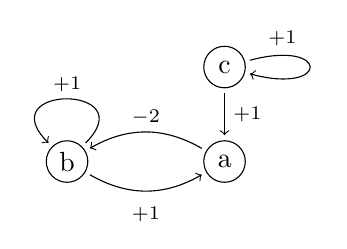
\begin{tikzpicture}[grn]
  \path[use as bounding box] (-0.5,-0.75) rectangle (3.2,1.7);
  \node[inner sep=0] (a) at (2,0) {a};
  \node[inner sep=0] (b) at (0,0) {b};
  \node[inner sep=0] (c) at (2,1.2) {c};
  \path[->]
    (b) edge[bend right] node[elabel, below=-2pt] {$+1$} (a)
    (c) edge node[elabel, right=-2pt] {$+1$} (a)
    (a) edge[bend right] node[elabel, above=-5pt] {$-2$} (b)
    (b) edge[loop, min distance=30pt] node[elabel, above=-5pt] {$+1$} (b)
    (c) edge[loop right, min distance=30pt] node[elabel, above=0pt, xshift=-10] {$+1$} (c);
\end{tikzpicture}
}
\end{minipage}
\begin{minipage}{0.6\linewidth}
\centering
\modMF{
\begin{align*}
  K_{a,\emptyset} &= 0 & K_{b,\emptyset} &= 0 \\
  K_{a,\{b\}} &= 1 & K_{b,\{a\}} &= 0 \\
  K_{a,\{c\}} &= 1 & K_{b,\{b\}} &= 1 \\
  K_{a,\{b,c\}} &= 2  & K_{b,\{a,b\}} &= 0 \\
  \\
  K_{c,\emptyset} &= 0 & K_{c,\{c\}} &= 1
\end{align*}
}
\end{minipage}
\caption{\label{fig:runningBRN}
  (left)
  IG example.
  Components are represented by nodes labeled with a name
  and regulations by edges labeled with their sign and threshold.
  For instance, the edge from $b$ to $a$ is labeled $+1$, which stands for: $\GRNedgef{b}{+}{1}{a}$.
  This means that if the expression level of $b$ is equal to (\ie above) 1, then $b$ activates $a$;
  otherwise, $b$ inhibits $a$.
  (right)
  Example parametrization on the left IG.
}
\end{figure}

A \emph{state} $s$ of an IG $(\Gamma, E)$ is an element in $\GRNstates \DEF \prod_{a \in \Gamma} \segm{0}{l_a}$.
$\GRNget{s}{a}$ refers to the level of component $a$ in $s$.
For each possible state, the set of \emph{resources} of a given component
is the set of regulators of this component whose expression level is above the threshold of the regulation (\pref{def:resources}).
In other words, in every state $s$, a regulator $b$ of a component $a$
is either a resource (if $\GRNget{s}{b} \in \levels{b}{a}$)
or not a resource (if $\GRNget{s}{b} \in \ulevels{b}{a}$).
%For each possible state, all regulators of a component $a$ can be divided into
%\emph{activators} and \emph{inhibitors}, given their type of interaction and expression level,
%referred to as the \emph{resources} of $a$ in this state (\pref{def:resources}).
Relying on this observation, the specificity of Thomas's approach lies in the use of discrete \emph{parameters} to represent the
focal level interval towards which the component will evolve in every configuration of the resources (\pref{def:param}).

\begin{definition}[Resources ($\GRNreslabel$)]\label{def:resources}
For a given component $a \in \Gamma$ and a state $s \in \GRNstates$,
the set of regulators of $a$ whose level in $s$ is above the related threshold %to regulate $a$
is called the set of \emph{resources} of $a$ in $s$ and is noted $\GRNres{a}{s}$:
$$\GRNres{a}{s} \DEF \{ b \in \GRNreg{a} \mid \GRNget{s}{b} \in \levels{b}{a} \}$$
\end{definition}

\begin{definition}[Parameter $K_{a,\omega}$ and Parametrization $K$]\label{def:param}
For a given component $a \in \Gamma$, and $\omega \subset \GRNreg{a}$ a set of regulators of $a$,
the \emph{parameter} \modMF{$K_{a,\omega} \in \segm{0}{l_a}$ is a non-negative integer}.
The complete map $K$ of parameters on $\IG$ is called a \emph{parametrization} on $\IG$.
\end{definition}

%\todo{Discuss on the widespread use of discrete parameters + binary resources}
An IG and a parametrization make up a complete BRN.
%The purpose of intervals as parameters is discussed at the end of this section.
%Regarding the dynamics, an interval parameter $K_{a,\omega}$ is the set of values towards which $a$ will tend
%in the states where its resources are exactly the regulators in $\omega$.
\modMF{Regarding the dynamics, a parameter $K_{a,\omega}$ is the value towards which $a$ will tend
in the states where its resources are exactly the regulators in $\omega$.}
%as defined in the asynchronous dynamics of \pref{def:dynamics}.
%At last, \pref{def:dynamics} gives the asynchronous dynamics of a BRN using Thomas' parameters.
Indeed, from a given state $s$, a transition to another state $s'$ is possible provided that
exactly one component $a$ evolves of one expression level \modMF{towards} $K_{a,\GRNres{a}{s}}$,
as stated by the definition of the transition relation $\GRNtrans{s}{s'}$ (\pref{def:dynamics}).
However, $a$ cannot evolve if its expression level already \modMF{equals}
the parameter $K_{a,\GRNres{a}{s}}$.

\begin{definition}[Asynchronous dynamics ($\GRNtrans{}{}$)]\label{def:dynamics}
The dynamics of a BRN using Thomas's parameters is given by the transition relation $\GRNtrans{}{}\ \in \GRNstates \times \GRNstates$ defined by:
\begin{align*}
  \forall s, s' \in \GRNstates, \GRNtrans{s}{s'} &\Longleftrightarrow \exists a \in \Gamma,
  \GRNget{s}{a} \neq K_{a, \GRNres{a}{s}} \wedge \GRNget{s'}{a} = \GRNget{s}{a} + \delta^a(s) \\
    & \qquad\quad \wedge \forall b \in \Gamma, b \neq a \Rightarrow \GRNget{s}{b} = \GRNget{s'}{b}
\end{align*}
with: $\delta^a(s) =
  \begin{cases}
    +1 & \text{if } \GRNget{s}{a} < K_{a, \GRNres{a}{s}} \\
    -1 & \text{if } \GRNget{s}{a} > K_{a, \GRNres{a}{s}} \\
  \end{cases}$
\end{definition}

\begin{example}
\pref{fig:runningBRN}(right) gives a Parametrization on the IG of \pref{fig:runningBRN}(left).
In this BRN, the following transitions are possible given the semantics defined in \pref{def:dynamics}:
$$\GRNstate{a_0, b_1, c_1} \rightarrow \GRNstate{a_1, b_1, c_1} \rightarrow \GRNstate{a_2, b_1, c_1} \rightarrow
\GRNstate{a_2, b_0, c_1} \rightarrow \GRNstate{a_1, b_0, c_1} \enspace,$$
where $a_i$ denotes the component $a$ at level $i$.
This sequence of states ends in a steady state: no evolution is possible in $\GRNstate{a_1, b_0, c_1}$.
\end{example}

\begin{remark}[Parameters equivalence]
\label{rem:K-equiv}
\modLP{%
In the scope of the asychronous dynamics (\pref{def:dynamics}), one can remark
that some parameters values can be equivalent, \ie the resulting dynamics is
the same.
It is notably the case with self-regulations:
if $\GRNedge{a}{s}{t}{a}$,
then for any $\omega\subseteq \GRNreg{a}$,
two values $v$ and $v'$ of the parameter 
$K_{a,\omega\setminus \{a\}}$ are equivalent
if $v\geq t$ and $v'\geq t$.
Similary,
two values $v$ and $v'$ of the parameter
$K_{a,\omega\cup\{a\}}$ are equivalent 
if $v<t$ and $v'<t$.}
\end{remark}


\paragraph{Interaction Graph of the dynamics}
From the dynamics specification of a BRN, one can infer back the IG that contain only the functional
regulations.
Let us define
$f^a(s) = s[a]$ if $s[a] = K_{a, \GRNres{a}{s}}$
and
$f^a(s) = s[a]+\delta^a(s)$ otherwise.
A positive (resp. negative) interaction from $b$ to $a$ is inferred if there exists a state $s$ such
that increasing $b$ in $s$ would increase (resp. decrease) $f^a$; in other words, if
there exists a state $s$ so that:
$f^a(s\{b_i\}) < \text{(resp. $>$) } f^a(s\{b_{i+1}\})$, 
where $i < l_b$ and $s\{b_i\}$ denotes the state $s$ where the component $b$ is assigned to $i$.
\modLP{If all the interactions from $b$ to $a$ are positive (resp. negative), there is a positive
(resp. negative) edge from $b$ to $a$ in the IG, denoting a monotonous influence of $b$ on $a$.
In the case when there exists two differently signed interactions, the edge in the IG is said
non-monotonous.
This abstract representation of the dynamical system can then} be used to derive global properties on
the dynamics (\eg \cite{Richard2010378,PR11-SASB}).



% vim:spell spelllang=en:
\section{Interaction Graph Inference from Process Hitting}\label{sec:infer-IG}

\todo{In this while section: add informal explanations and maybe more examples.\\
Especially:
\begin{itemize}
  \item Intuitively detail the motivations
  \item Give the intuition of the methods (esp. $\focals$)
  \item Insist on the use/motivation of the definitions
\end{itemize}
The reviewer also proposes to use a biological running example (such as $\lambda$-phage).}

The Interaction Graph (IG) is an abstract representation of the direct qualitative influences,
positive and/or negative, between the components of the system.
As discussed in \pref{sec:intro}, the IG allows to efficiently characterize global dynamical
properties for the concrete system, such as the capability for multi-stationarity or oscillation.

\todo{The reviewer says about the following paragraph: “The inference of an
IG from a dynamics is interesting and important in biology. However the
motivations expressed here are not well argued. In particular I don't find
this “common”. Some bibliographical references are required to consolidate
the arguments or the sentence has to be rephrased.”}

In a typical biological network modeling process, a prior IG is generally the starting point for
the formal system specification.
However, it is common that the prior IG actually refers to interactions that reveal to be 
non-effective with respect to the dynamics.
Hence, deriving the IG directly from the dynamical models lead to more concise IGs, enhancing the
conclusiveness of static analyses based upon this abstract representation.

In this section, we formally derive the IG corresponding to a given PH that is well-formed for BRN
modeling.
This section first introduces the notion of focal processes within a PH (\pref{ssec:focal})
which is used to characterize well-formed PH for IG inference (\pref{ssec:wf}).
%and as well used by the parametrization inference presented in \pref{sec:infer-K}.
The rules for inferring the interactions between components from a PH are
described in \pref{ssec:infer-IG}.
We consider hereafter a global PH $(\PHs,\PHl,\PHa)$ on which the IG inference is to be
performed.


\subsection{Well-formed Process Hitting for Interaction Graph Inference}\label{ssec:wf}

\todo{rework text with new paper structure (\pref{sec:tr2global})}

The inference of an IG from a PH assumes that the PH defines two types of sorts:
the sorts corresponding to BRN components, and the cooperative sorts.
This leads to the characterization of a \emph{well-formed} PH for IG inference.

The identification of sorts modeling components relies on the observation that their processes
represent (ordered) qualitative levels.
Hence an action on such a sort cannot make it bounce to a process at a distance more than one.
The set of sorts satisfying such a condition is referred to as $\Gamma$
(\pref{eq:PH-components}).
Therefore, in the rest of this paper, $\Gamma$ denotes the set of components of the BRN to infer.

\begin{equation}
\Gamma \DEF \{a \in \PHs \mid \nexists \PHfrappe{b_i}{a_j}{a_k} \in \PHa, |j - k| > 1\} \\
\label{eq:PH-components}
\end{equation}

\todo{maybe we should also support a user-supplied $\Gamma$ and give the
constraints (included in the prev. def?)}


Finally, \pref{pro:wf-ph} sums up the conditions for a Process Hitting to be suitable for IG
inference.
In addition of having either component sorts or well-formed cooperative sorts, we also require that
there is no cycle between cooperative sorts, and that
sorts being never hit (\ie serving as an invariant environment) are components.

\begin{property}[Well-formed Process Hitting for IG inference]\label{pro:wf-ph}
A PH is well-formed for IG inference if and only if the following conditions are verified:
\begin{itemize}
\item 
each sort $a\in\PHs$ either belongs to $\Gamma$, or is a well-formed cooperative sort;
\item 
there is no cycle between cooperative sorts
(the digraph $(\Sigma,\{(a,b)\in(\Sigma\times\Sigma)\mid \exists \PHfrappe{a_i}{b_j}{b_k}\in\PHa
\wedge a\neq b\wedge \{a,b\}\cap\Gamma=\emptyset \})$ is
acyclic);
\item 
sorts having no action hitting them belong to $\Gamma$
($\{ a \in \Sigma\mid \nexists \PHfrappe{b_i}{a_j}{a_k}\in\PHa\} \subset \Gamma$).
\end{itemize}
\end{property}

\begin{example}
In the PH of \pref{fig:runningPH-2}, $bc$ is a well-formed cooperative sort as defined in \pref{pro:wf-cooperative-sort}, because:
\begin{align*}
\focals(bc, \PHl_{bc}, \{b_0, c_0\} \cup \PHl_{bc}) = \{bc_{00}\} && \focals(bc, \PHl_{bc}, \{b_0, c_1\} \cup \PHl_{bc}) = \{bc_{01}\} \\
\focals(bc, \PHl_{bc}, \{b_1, c_0\} \cup \PHl_{bc}) = \{bc_{10}\} && \focals(bc, \PHl_{bc}, \{b_1, c_1\} \cup \PHl_{bc}) = \{bc_{11}\}
\end{align*}
Hence, both \pref{fig:runningPH-1} and \pref{fig:runningPH-2} are well-formed PH for IG inference
with $\Gamma = \{a,b,c\}$.
\end{example}



\subsection{Interaction Inference}\label{ssec:infer-IG}

At this point we can divide the set of sorts $\PHs$ into components ($\Gamma$, see \pref{eq:PH-components}) and cooperative sorts
that will not appear in the IG ($\PHs \setminus \Gamma$).
We define in \pref{eq:ph_predec} the set of predecessors of a sort $a$, that is, the sorts influencing $a$
by considering direct actions and possible intermediate cooperative sorts.
The predecessors of $a$ that are components are the regulators of $a$, denoted $\PHpredecgene{a}$
(\pref{eq:regulators}).
\begin{align}
\begin{split}
\forall a \in \PHs, \PHpredec{a} &\DEF \{b \in \PHs \mid \exists n \in \mathbb{N}^*, \exists
(c^k)_{k \in \segm{0}{n}} \in \PHs^{n+1}, \\
                                   & \quad \quad c^0 = b \wedge c^n = a \\
                                   & \quad \quad \wedge \forall k \in \segm{0}{n-1},
                   c^k \in \PHdirectpredec{c^{k+1}} \cap (\PHs\setminus\Gamma)\}
\end{split}
\label{eq:ph_predec}
\\
\forall a\in \PHs, \PHpredecgene{a} & \DEF \PHpredec{a} \cap \Gamma
\label{eq:regulators}
\end{align}

Given a set $g$ of components and a configuration (\ie a sub-state) $\sigma$, $\ctx_g(\sigma)$
refers to the set of processes hitting $a$ regulated by any sort in $g$ (\pref{eq:ctx-sigma}).
If $g=\{b\}$, we simply note $\ctx_b(\sigma)$.
This set is composed of the active processes of sorts in $g$, and the focal process (assumed
unique) of the cooperative sorts $\upsilon$ hitting $a$ that have a predecessor in $g$.
The evaluation of the focal process of $\upsilon$ in context $\sigma$, denoted $\upsilon(\sigma)$,
relies on \pref{pro:wf-cooperative-sort}, which gives its value when all the direct predecessors of
$\upsilon$ are defined in $\sigma$.
When a predecessor $\upsilon'$ is not in $\sigma$, we extend the evaluation by recursively computing
the focal value of $\upsilon'$ is $\sigma$, as stated in \pref{eq:cooperative-eval},
where $\uplus$ stands for a union of states (which are sets of processes).
Because there is no cycle between cooperative sorts, this recursive evaluation of $\upsilon(\sigma)$
always terminates.
\begin{align}
\forall g\subset \Gamma,
  \ctx_g(\sigma) & \DEF \{ \sigma[b] \mid b\in g \} \cup \{ \upsilon(\sigma) \mid
\upsilon\in\PHdirectpredec{a} \setminus \Gamma \wedge g\cap \PHpredecgene{\upsilon} \neq \emptyset \}
\label{eq:ctx-sigma}
\\
\upsilon(\sigma) & \DEF
\upsilon(\sigma \uplus \state{\upsilon'(\sigma) \mid 
  \upsilon'\in\PHdirectpredec{\upsilon} \wedge
  \upsilon'\in\PHs\setminus\Gamma })
\label{eq:cooperative-eval}
\end{align}

This inference mainly focuses on the presence of actions betweens two sorts to conclude on the presence of a regulation.
We aim at inferring that $b$ activates (inhibits) $a$ if there exists a configuration where increasing
the level of $b$ makes possible the increase (decrease) of the level of $a$,
which is directly inspired from the works of~\cite{Richard2010378}.
To do so, the sets of components cooperating together to hit $a$, called groups of influence of $a$, are studied.
Such groups are given by $X(a)$ which is the set of connected components in the graph linking two regulators
$b$ and $c$ of $a$ if they use a common cooperative sort to have an influence on $a$ (\pref{eq:influence-groups}).
\begin{equation}
X(a) = \mathcal C\left( (\PHpredecgene{a}, \{ \{b,c\} \mid
        \exists \upsilon\in \PHdirectpredec{a} \setminus \Gamma,
        \{b,c\} \subset \PHpredecgene{\upsilon} \}) \right)
\label{eq:influence-groups}
\end{equation}

\def\fp{\Phi}


\modLP{
\begin{equation}
\fp(a_i) \DEF \{\sigma\in L(\PHpredecgene{a}\cup\{a\}) \mid \sigma[a] = i \wedge
					\focals(a, \{a_i\}, \ctx_{\PHpredecgene{a}}(\sigma)) =
					\{a_i\} \}
\label{eq:fp}
\end{equation}
}


To infer influence of a component $b$ on a component $a$,
we observe the direction of evolution of $a$ for different active processes of $b$.
The fact that $a$ tends to evolve differently when $b$ changes denotes an influence from $b$.
Formally, for a given group $g$ of regulators of a component $a$
(that is, a minimal set of components regulating $a$ through common cooperative sorts),
and a configuration $\ctx$ on $g$, we note
$\irB_a(\sigma)$ the set of processes towards which $a$ can bounce (\pref{eq:possible-bounces}).
%This set is defined using the set $\irF_a(\sigma)$ of action hitting $\PHget{\sigma}{a}$ in $\sigma$ (\pref{eq:possible-actions})
%and the set of processes $\ctx$ hitting any process of $a$ (\pref{eq:ctx-sigma}).
If $a$ cannot be hit by any action in $\sigma$, then $\irB_a(\sigma) = \{ \PHget{\sigma}{a} \}$.
%

\modLP{
$\forall g\in X(a), \forall \sigma\in L(g\cup\{a\}), i=\sigma[a]$:
\begin{align}
a_i \in \irB_a^g(\sigma) &\EQDEF \exists\sigma'\in\fp(a_i): \sigma\subset\sigma'
\label{eq:B-no-bounce}
\\
\forall a_j\in L_a, j\neq i,
a_j \in \irB_a^g(\sigma) &\EQDEF \focals(a, \{a_j\}, \ctx_{g}(\sigma)) = \{a_j\}
\label{eq:B-bounce}
\end{align}}

\pref{pps:inference-edges} details the inference of all existing influences between components occurring
with a threshold $t$.
The main idea of this inference is that
the presence of a positive (negative) influence of a component $b$ on $a$ denotes the fact that
there exists a state in which increasing the level of $b$ tends to make the future level of $a$ rise (drop)
(\pref{eq:edges-inference}).
Therefore, these influences are split into positive and negative ones, and represent possible edges in the final IG.
Furthermore, studying the influences of the groups of regulators of $a$
allows to study its auto-influences, and thus infer auto-edges on $a$ in the IG (\pref{eq:edges-inference-auto}).
Finally, \pref{eq:edges-inference-noreg} handles the special case where $a$ has no regulators.
We ignore the cases where a component has no visible influence on another.
%
\begin{proposition}[Influences inference]\label{pps:inference-edges}
We define the set of positive (resp. negative) influences $\hat{E}_+$ (resp.
$\hat{E}_-$) by
\modLP{
\begin{align}
\begin{split}
\forall a\in\Gamma, \forall b\in\PHpredecgene{a}, b\neq a, & \forall s \in \{ +, - \}, \\
  b \xrightarrow{t+1} a \in \hat{E}_s \EQDEF & \exists g \in X(a), 
  	b \in g, \exists \sigma \in L(g\cup\{a\}), \\
    \qquad & \{ b_t, b_{t+1} \} \subset \PHl_b \wedge b_t \in \sigma,\\
    \qquad & \exists a_j \in \irB_a^g(\sigma), \exists a_k \in \irB_a^g(\sigma\{b_{t+1}\}), \\
	\qquad & k > j \wedge s=+  \vee j < t \wedge s=-
\end{split}
\\
\begin{split}
 \forall a\in\Gamma: a\in\PHpredecgene{a}, & \forall s \in \{ +, - \}, \\
  b \xrightarrow{t+1} a \in \hat{E}_s \EQDEF & \exists g \in X(a), 
  	b\neq a \Rightarrow b \in g, \exists \sigma \in L(g\cup\{a\}), \\
    \qquad & \{ b_t, b_{t+1} \} \subset \PHl_b \wedge b_t \in \sigma,\\
    \qquad & \exists a_j \in \irB_a^g(\sigma), \exists a_k \in \irB_a^g(\sigma\{b_{t+1}\}), \\
	\qquad & k\geq t+1 \wedge j \leq t \wedge s=+ \\
	\qquad & \vee k<t+1 \wedge j>t \wedge s=-
\end{split}
\\
\forall a\in\Gamma: \PHpredecgene{a} = \emptyset, &
	\forall t\in\{0,\cdots,l_a-1\},
	a \xrightarrow{t+1} a \in \hat{E}_+
\end{align}
}
\end{proposition}

We are now able to infer the edges of the final IG by considering positive and negative influences
(\pref{pps:inference-IG}).
We infer a positive (resp. negative) edge if there only exist corresponding influences with the same sign.
If an influence is both positive and negative, we infer an unsigned edge.
In the end, the threshold of each edge is the minimum threshold for which an influence has been found.
%
\begin{proposition}[Interaction Graph inference]\label{pps:inference-IG}
We infer $\IG = (\Gamma,E)$ using \pref{pps:inference-edges} as follows:
\begin{align*}
E_+ &= \{ \GRNedge{a}{+}{t}{b} \mid \nexists a \xrightarrow{t'} b \in \hat{E}_-
  \wedge t = \min \{ l \mid a \xrightarrow{l} b \in \hat{E}_+\}\} \\
E_- &= \{ \GRNedge{a}{-}{t}{b} \mid \nexists a \xrightarrow{t'} b \in \hat{E}_+
  \wedge t = \min \{l \mid a \xrightarrow{l} b \in \hat{E}_-\}\} \\
E_\pm &= \{ \GRNedge{a}{\uns}{t}{b} \mid \exists a \xrightarrow{t'} b \in \hat{E}_+ \wedge \exists a \xrightarrow{t''} b \in \hat{E}_- \\
  & \qquad\qquad\qquad \wedge t = \min \{l \mid a \xrightarrow{l} b \in \hat{E}_- \cup \hat{E}_+\}\}
\end{align*}
\end{proposition}



\begin{example}
The IG inference of the PH of \pref{fig:runningPH-2} gives the
IG in \pref{fig:BRN-inf1}, containing the following edges:
\begin{align*}
  E_+ &= \{\GRNedgef{b}{+}{1}{a}, \GRNedgef{c}{+}{1}{a}, \GRNedgef{a}{+}{1}{a}, \GRNedgef{b}{+}{1}{b}, \GRNedgef{c}{+}{1}{c}\}\\
  E_- &= \{\GRNedgef{a}{-}{2}{b}\} \qquad\qquad\qquad\qquad\qquad
  E_\uns = \emptyset
\end{align*}
This IG is close to the one in \pref{fig:runningBRN} but not equivalent,
as each component has an additional auto-action.
The auto-actions on $b$ and $c$ are the consequence of a global stability
in some configurations: $c$ never evolves, and neither does $b$ when $a_2$ is not active.
The auto-action on $a$ is mainly caused by its multi-valued nature.

The inference of the PH of \pref{fig:runningPH-1}
(without refinement with cooperative sort) gives the same IG.

\begin{figure}[t]
\centering
\scalebox{1.2}{
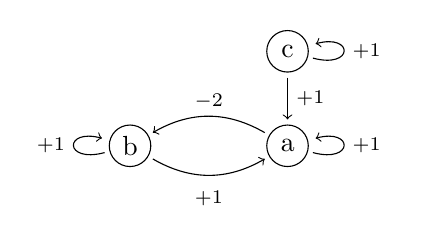
\begin{tikzpicture}[grn]
  \path[use as bounding box] (-1.3,-0.75) rectangle (3.5,1.5);
  \node[inner sep=0] (a) at (2,0) {a};
  \node[inner sep=0] (b) at (0,0) {b};
  \node[inner sep=0] (c) at (2,1.2) {c};
  \path[->]
    (b) edge[bend right] node[elabel, below=-2pt] {$+1$} (a)
    (c) edge node[elabel, right=-2pt] {$+1$} (a)
    (a) edge[bend right] node[elabel, above=-5pt] {$-2$} (b)
    (b) edge[in=-15+180, out=15+180, loop] node[elabel, left=-2pt] {+1} (b)
    (c) edge[in=15, out=-15, loop] node[elabel, right=-2pt] {+1} (c)
    (a) edge[in=15, out=-15, loop] node[elabel, right=-2pt] {+1} (a);
\end{tikzpicture}
}
\caption{\label{fig:BRN-inf1}
  Result of the IG inference performed on the PH of \pref{fig:runningPH-2}.
}
\end{figure}

\end{example}



\begin{example}
If we add the action $\PHfrappe{a_2}{b_0}{b_1}$ to the PH of \pref{fig:runningPH-2},
then two unsigned edges towards $b$ are inferred instead of the previous signed edges:
\begin{align*}
  E_+ &= \{\GRNedgef{b}{+}{1}{a}, \GRNedgef{c}{+}{1}{a}, \GRNedgef{a}{+}{1}{a}, \GRNedgef{c}{+}{1}{c}\}\\
  E_- &= \emptyset \qquad\qquad\qquad\qquad
  E_\uns = \{\GRNedgef{a}{\uns}{2}{b}, \GRNedgef{b}{\uns}{1}{b}\}
\end{align*}
This is due to the fact that the actions $\PHfrappe{a_2}{b_1}{b_0}$ and $\PHfrappe{a_2}{b_0}{b_1}$
introduce an oscillation only caused by $a$, which cannot be represented in Thomas modeling.
\end{example}

\section{Parametrization inference}\label{sec:infer-K}

\todo{In this while section: add informal explanations and maybe more examples (see previous section).}

Given the IG inferred from a PH as presented in the previous section, one can find the discrete parameters
that model the behavior of the studied PH using the method presented in the following.
It relies on an exhaustive enumeration of all predecessors of each component in order to find attractor processes
and returns a possibly incomplete parametrization, given the exhaustiveness of the cooperations (\pref{ssec:infer-K}).
The last step consists of the enumeration of all compatible complete parametrizations (\pref{ssec:admissible-K}) given this
set of inferred parameters, the PH dynamics and some biological constraints on parameters.

\subsection{Parameters inference}\label{ssec:infer-K}

This subsection presents some results related to the inference of independent discrete parameters from a given PH.
These results are equivalent to those presented in \cite{PMR10-TCSB}, with notation adapted to be shared with the previous section.
In addition, we introduce the well-formed PH for parameter inference property (\pref{pro:wf-ph-K}),
which implies that %the inferred IG does not contain any unsigned interactions, and thus can be seen as the
%regular IG $(\Gamma, E)$,
%and that 
any process in $\levels{b}{a}$ (resp. $\ulevels{b}{a}$) share the same behavior
regarding $a$.

\todo{makes it standalone: repeat the constraints for IG inference that are
actually necessary + check that we can do if if the IG is provided (then what
are the constraints on this IG)}

\begin{property}[Well-formed PH for parameter inference]\label{pro:wf-ph-K}
A PH is well-formed for parameter inference if and only if
it is well-formed for IG inference, and
the IG $(\Gamma, E)$ inferred by \pref{pps:inference-IG}
verifies the following property:
\todo{Define $c(\sigma)$ for $\sigma \in \textstyle\prod_{d \in \PHpredec{c}} \PHl_d$
(\ie the unique focal point)}
\begin{align*}
  \begin{split}
%   \forall a \in \Gamma&, \forall b\in \GRNreg{a},
%           \forall (i,j\in\levels{b}{a} \vee i,j\in\ulevels{b}{a}), \\
%   & \quad \forall c \in \PHs, ( (b\neq a\wedge c=a) \vee (c\in\PHpredec{a}\setminus \Gamma \wedge b\in\PHdirectpredec{c})), \\
%   & \qquad
%                           \PHfrappe{b_i}{c_k}{c_l}\in\PHa \Leftrightarrow
%                                   \PHfrappe{b_j}{c_k}{c_l}\in\PHa
      &
    \forall a \in \Gamma,
    \forall g \in X(a),
    \forall \sigma, \sigma' \in \textstyle\prod_{d \in g} \PHl_d,
    \forall b \in g,
    b \in \GRNreg{c},
    \forall c \in \PHdirectpredec{a} \setminus \Gamma,
      \\&\qquad
    b \in \reg{c},
    \forall (i,j \in \levels{b}{a} \vee i,j \in \ulevels{b}{a}),
%    \forall b_i \in \PHl_b,
    b_i \in \sigma,
%    b_i \in \levels{b}{a},
%    \forall b_j \in \levels{b}{a},
      \\&\qquad\qquad
    \sigma' = \sigma\{b_j\},
    %c_{\sigma} \in \PHl_c \wedge c_{\sigma'} \in \PHl_c,  %facultatif
    \PHfrappe{c(\sigma)}{a_i}{a_j} \in \PHa \Leftrightarrow
    \PHfrappe{c(\sigma')}{a_i}{a_j} \in \PHa
  \end{split}\\
  \begin{split}
    & \forall a \in \Gamma, \forall b \in \GRNreg{a},
      \forall (i,j \in \levels{b}{a} \vee i,j \in \ulevels{b}{a}), \\
    & \qquad \forall c \in \PHs, b \neq a,
      \PHfrappe{b_i}{a_k}{a_l} \in \PHa \Leftrightarrow
      \PHfrappe{b_j}{a_k}{a_l} \in \PHa
  \end{split}
\end{align*}
\end{property}

Let $K_{a,\omega}$ be the parameter we want to infer for a given component $a \in \Gamma$
and $\omega \subset \GRNreg{a}$ a set of its regulators.
This inference, as for the IG inference, relies on the search of focal processes of the component for the given configuration of its regulators.

For each sort $b \in \GRNreg{a}$, we define a context $C^b_{a,\omega}$ in \pref{eq:param_context} that contains all processes representing the influence of the resources in the configuration modeled by $\omega$.
The context of a cooperative sort $\upsilon$ that regulates $a$ is given in
\pref{eq:param_context_coop} as the set of focal processes matching the current configuration.
$C_{a,\omega}$ refers to the union of all these contexts (\pref{eq:K-ctx}).
\begin{align}
  \label{eq:param_context}
  \forall b\in\Gamma,~
  C_{a,\omega}^b & \DEF \begin{cases}
    \levels{b}{a} & \text{if $b \in \omega$,}\\
    \ulevels{b}{a} & \text{if $b \notin \omega$,}\\
    L_b            & \text{otherwise;}\\
  \end{cases}
  \\
  \label{eq:param_context_coop}
  \forall \upsilon \in \PHpredec{a}\setminus\Gamma,~
  C_{a,\omega}^\upsilon & \DEF \{
  \upsilon(\sigma) \mid \sigma \in \textstyle\prod_{c\in\PHdirectpredec{\upsilon}}C_{a,\omega}^c \}
  \\
  C_{a,\omega} & \DEF \textstyle\bigcup_{b\in\PHpredec{a}} C^b_{a,\omega}
  \label{eq:K-ctx}
\end{align}

The parameter $K_{a,\omega}$ specifies to which values $a$ eventually evolves as long as the context
$C_{a,\omega}$ holds, which is precisely the definition of the $\focals$ function
(\pref{def:focals} in \pref{ssec:focal}),
where the focals reachability property can be derived from \pref{pro:wf-ph-K} and
\pref{eq:param_context_coop}.
Hence $K_{a,\omega} = \focals(a,C^a_{a,\omega},C_{a,\omega})$ if this latter is a non-empty interval
(\pref{pps:param_K}).

\begin{proposition}[Parameter inference]
\label{pps:param_K}
Let $(\PHs, \PHl, \PHh)$ be a Process Hitting well-formed for parameter inference, and $\IG = (\Gamma, E)$ the inferred IG.
Let $A$ (resp. $B$) $\subseteq \Gamma$ be the set of regulators that activate (resp. inhibit) a sort
$a$.
If $\focals(a,C^a_{a,\omega},C_{a,\omega})=\segm{a_i}{a_j}$ is a non-empty interval, then $K_{a,\omega} = \segm{i}{j}$.
\end{proposition}

\begin{example}
\label{ex:infer-param-runningPH-1}

Applied to the PH in \pref{fig:runningPH-1}, we infer the following parameters:
\begin{align*}
K_{a, \emptyset} &= \segm{0}{0} &
K_{b, \emptyset} &= \segm{0}{0} \\
K_{a, \{a\}} &= \segm{0}{0} &
K_{b, \{a\}} &= \segm{0}{0} \\
K_{a, \{c\}} &= \segm{1}{1} &
K_{b, \{b\}} &= \segm{1}{1} \\
K_{a, \{b\}} &= \segm{1}{1} &
K_{b, \{a,b\}} &= \segm{0}{0} \\
K_{a, \{b,c\}} &= \segm{1}{1} &
K_{c, \emptyset} &= \segm{0}{0} \\
K_{a, \{a,b,c\}} &= \segm{2}{2} &
K_{c, \{c\}} &= \segm{1}{1}
%K_{a, \{a,b\}} = ?
%K_{a, \{a,c\}} = ?
\end{align*}
$K_{a,\{a,b\}}$ and $K_{a,\{a,c\}}$ cannot be inferred,
which is a direct consequence of the lack of cooperation between $b$ and $c$ on $a$.
\end{example}

\begin{example}
Regarding the refined PH of \pref{fig:runningPH-2}, all parameters can be inferred.
We obtain the same value for the inferred parameters of \pref{ex:infer-param-runningPH-1},
together with the following results:
\begin{align*}
  K_{a,\{a,b\}} &= \segm{1}{1} &
  K_{a,\{a,c\}} &= \segm{1}{1}
\end{align*}
\end{example}

Given the \pref{pps:param_K}, we see that in some cases, the inference of the targeted parameter is impossible.
This can be due to a lack of cooperation between regulators:
when two regulators independently hit a component, their actions can have opposite effects, leading to two possible evolutions.
Such an indeterminism is not possible in Thomas modeling as in a given configuration of regulators,
a component can only have an interval attractor, and can therefore evolve in only one direction.
In order to avoid such inconclusive cases, one has to ensure that no such behavior is allowed by
either removing undesired actions or using cooperative sorts to prevent opposite influences between
concurrent regulators.

\subsection{Admissible parametrizations}\label{ssec:admissible-K}

When building a BRN, one has to find the parametrization that best describes the desired behavior of the studied system.
Complexity is inherent to this process as the number of possible parametrizations for a given IG is exponential w.r.t.~the number of components.
However, the method of parameters inference presented in this section gives some information about necessary parameters given a certain dynamics described by a PH.
This information thus drops the number of possible parametrizations, allowing to find the desired behavior more easily.

We first delimit the validity of a parameter (\pref{pro:K-valid}) in order to ensure that any
transition in the resulting BRN is allowed by the studied PH.
This is verified by the existence of a hit making the concerned component bounce into the direction
of the value of the parameter in the matching context.
Thus, assuming \pref{pro:wf-ph-K} holds, any transition in the inferred BRN corresponds to at least
one transition in the PH, proving the correctness of our inference.
We remark that any parameter inferred by \pref{pps:param_K} satisfies this property.

\begin{property}[Parameter validity]\label{pro:K-valid}
A parameter $K_{a,\omega}$ is valid w.r.t. the PH if and only if the following equation is verified:
\begin{align*}
  \forall a_i\in C^a_{a,\omega}, a_i \notin K_{a,\omega} \Longrightarrow
    (& \exists \PHfrappe{c_k}{a_i}{a_j}\in\PHa, c_k \in C^c_{a,\omega} \\
     & \wedge a_i < K_{a,\omega} \Rightarrow j > i \wedge  a_i > K_{a,\omega} \Rightarrow j <i )
\end{align*}
\end{property}

Then, we use some additional biological constraints on Thomas' parameters given in
\cite{BernotSemBRN}, that we sum up in the following three properties:

\begin{property}[Extreme values assumption]
Let $\IG = (\Gamma, E)$ be an IG. A parametrization $K$ on $\IG$ satisfies the \emph{extreme values assumption} if and only if:
\label{pro:param_enum_extreme}
\begin{align*}
  \forall b \in \Gamma, \GRNreg{b} \neq \emptyset \Longrightarrow \exists \omega \subset \GRNreg{b}, 0 \in K_{b,\omega} \wedge \exists \omega' \subset \GRNreg{b}, l_b \in K_{b,\omega'}
\end{align*}
\end{property}

\begin{property}[Activity assumption]
\label{pro:param_enum_activity}
Let $\IG = (\Gamma, E)$ be an IG. A parametrization $K$ on $\IG$ satisfies the \emph{activity assumption} if and only if:
\begin{align*}
  \forall b \in \Gamma, \forall a \in \GRNreg{b}, \exists \omega \subset \GRNreg{b}, K_{b,\omega} \neq K_{b,\omega \cup \{ a \}}
\end{align*}
\end{property}

\begin{property}[Monotonicity assumption]
\label{pro:param_enum_monotonicity}
Let $\IG = (\Gamma, E)$ be an IG. A parametrization $K$ on $\IG$ satisfies the \emph{monotonicity assumption} if and only if:
\begin{align*}
  \forall b \in \Gamma,
  \forall A^+ \subset \{ a \in \Gamma \mid \GRNedge{a}{+}{t}{b} \in E_+ \}&,
  \forall A^- \subset \{ a \in \Gamma \mid \GRNedge{a}{-}{t}{b} \in E_- \},\\
  K_{b,\omega \cup A^-} & \leqsegm K_{b,\omega \cup A^+}
\end{align*}
\end{property}

\begin{example}\label{ex:enum-param-runningPH-1}
The parametrization inferred in \pref{ex:infer-param-runningPH-1} was partial because $K_{a,\{a,b\}}$ and $K_{a,\{a,c\}}$ could not be inferred.
It is however possible to enumerate all complete and admissible parametrizations
compatible with both the inferred parameters, and the properties of this subsection.
This enumeration gives 9 different parametrizations which correspond to the 3 possible values
for each of the two parameters that could not be inferred:
\begin{align*}
  K_{a,\{a,b\}} &\in \{ \segm{1}{1}, \segm{1}{2}, \segm{2}{2} \} \\
  K_{a,\{a,c\}} &\in \{ \segm{1}{1}, \segm{1}{2}, \segm{2}{2} \}
\end{align*}
We note that for all solutions, $0 \notin K_{a,\{a,b\}} \wedge 0 \notin K_{a,\{a,c\}}$.
This is due to the monotonicity assumption (\pref{pro:param_enum_monotonicity}) which especially states that:
\begin{align*}
  K_{a,\{b\}} \leqsegm K_{a,\{a,b\}} \wedge
  K_{a,\{c\}} \leqsegm K_{a,\{a,c\}}
\end{align*}

Finally, we note that $\segm{1}{1}$ belongs to the possible values for both parameters.
Therefore this enumeration allows, from the model in \pref{fig:runningPH-1},
to find the behavior of the model refined with a cooperative sort described in \pref{fig:runningPH-2}.
\end{example}

\section{Answer Set Programming implementation concepts}\label{sec:impl}

%\newcommand{\atom}{\mathbf}
\newcommand{\atom}[1]{#1}
%\newcommand{\predicate}{\mathbf}
\newcommand{\predicate}[1]{\mathit{#1}}
\newcommand{\la}{\leftarrow}
\newcommand{\var}[1]{#1}
\newcommand{\nota}{\neg}

\newcommand{\paramlabel}{\predicate{param\_label}}
\newcommand{\paramres}{\predicate{param\_resource}}
\newcommand{\component}{\predicate{component}}
\newcommand{\componentlevels}{\predicate{component\_levels}}
\newcommand{\param}{\predicate{param}}
\newcommand{\inferedparam}{\predicate{infered\_param}}
\newcommand{\lessactive}{\predicate{less\_active}}
\newcommand{\paraminf}{\predicate{param\_inf}}



Answer Set Programming (ASP) is a logic programming paradigm \cite{Baral03, Baral10},
which has been chosen to address the enumeration of all admissible parametrizations.
The motivations are following:
\begin{itemize}
  \item ASP efficiently tackles the inherent complexity of the used models, thus enabling us fast execution of the formal tools defined in this paper,
  \item ASP can efficiently enumerate a large set of possible answers,
  \item and it is easy to constrain the answers according to some properties.
\end{itemize}
We now synthesize some key points to better make the reader understand our ASP implementation with the enumeration example.



\subsection{Simple rules and answer sets}\label{sssec:simple_rules}
ASP is based on a set of rules of of the form:
\begin{align*}
  \underbrace{{\ }\atom{H}_{\ }}_{head} \la \underbrace{\atom{A}_1, \atom{A}_2, \dots, \atom{A}_n, \nota \atom{B}_1, \nota \atom{B}_2, \dots, \nota \atom{B}_m}_{body}.
\end{align*}
where the $body$ is a series of atoms ($\atom{A}_i$) and negations of atoms ($\nota \atom{B}_i$).
In the case of \emph{simple rules} (as opposed to the \emph{cardinality rules} of \pref{sssec:cardinality_rules}), the $head$ is also an atom ($\atom{H}$).
Such a rule, whose formal semantics is defined below,
schematically states that if all atoms $\atom{A}_1, \atom{A}_2, \dots, \atom{A}_n$ are true
and all atoms $\atom{B}_1, \atom{B}_2, \dots, \atom{B}_m$ are not true (negation by failure), then $\atom{H}$ has to be true.

An atom is composed of a predicate and a series of arguments (possibly empty).
For example, the following atom:
\begin{align*}
  \predicate{p}(x_1, x_2, \dots, x_r)
\end{align*}
is composed of the predicate $\predicate{p}$ and $r$ arguments: $x_1, x_2, \dots, x_r$.
Each argument is either a \emph{constant}, which is a representation of a piece of data (component name, expression level, …),
or a \emph{variable}, which is in fact a shorthand for any possible constants (variables are detailed below).
In this paper, constants are either numerical or consist of a single lowercase letter (\eg $a$, $b$, $c$, $1$, $2$, …)
while variables are always denoted by a single capital letter (\eg $\var{A}$, $\var{P}$, $\var{Q}$, …).
We do not use function symbols as arguments in this work.

\begin{example}\label{ex:asp-atom}
Consider a PH model such as depicted in \pref{fig:runningPH-1}:
in order to state the existence of each component, we use a predicate called $\component$ with two arguments:
\begin{align*}
  &\component(x, n).
\end{align*}
where $x$ is the name of the component and $l_x = n$ is its maximum expression level.
\end{example}

An ASP program is a set of rules as described above.
Solving an ASP program means finding an \emph{answer set}, which is a minimal set of atoms that respect all the rules.
In order to formally define this notion of answer set,
let us define a \emph{definite rule} as a rule with no negation of atoms (noted “$\nota$” above),
and a \emph{definite program} as a program containing only definite rules.
Let $S$ be a set of atoms: a definite rule is \emph{satisfied} by $S$ if $\atom{H} \in S$,
or if $\exists i \in \segm{1}{n}, A_i \notin S$.
Given this definition of satisfaction, we define the answer set of a definite program $\Pi$
as the (unique) minimal set $S$ of atoms that satisfies all the rules in $\Pi$.

In order to consider the general case,
for all non-definite program $\Pi$ and set $S$ of atoms, we denote $\Pi^S$ the reduct of $\Pi$ w.r.t.~$S$, defined from $\Pi$ by:
\begin{enumerate}
  \item deleting all the rules that have a negation of atom $\nota \atom{B}_i$ in the body where $\atom{B}_i \in S$, and
  \item removing all negations of atoms in the bodies of the remaining rules.
\end{enumerate}
Then, a set of atoms $S$ is an answer set of a non-definite program $\Pi$ if it is the answer set of $\Pi^S$, which is a definite program.
We note that several answer sets can be solution to the same non-definite program, and in practice a solver can be directed to enumerate them all.

%\begin{example}
%  As an example not related to the current work, consider the following ASP program:
%  \begin{align*}
%    a &\la \nota b.\\
%    b &\la \nota a.
%  \end{align*}
%  This program has the two following answer sets: $\{a\}$ and $\{b\}$.
%\end{example}



Note that it is possible to define a simple rule with no $body$ part.
Such a rule is called a \emph{fact}, and its $head$ atom consequently has to belong to all answer sets.
For instance, the information describing the studied model (the original PH model and the inferred IG and parameters) are expressed in ASP using facts.

\begin{example}\label{ex:asp-component}
In order to define the 3 components of \pref{fig:runningPH-1}, we use the following program:
\begin{align*}
  &\component(a, 2). \\
  &\component(b, 1). \\
  &\component(c, 1).
\end{align*}
This program contains only facts using the predicate $\component$ defined in \pref{ex:asp-atom},
and $a$, $b$, $c$, $1$ and $2$ are constants.
\end{example}



\subsection{Variables}
To describe the sets of all expression levels of each component (\ie the set $\segm{0}{l_a}$ for each $a \in \Gamma$),
one can use atoms of the form $\componentlevels(a, k)$ to state that $k \in \segm{0}{l_a}$.
Variables here come in handy to enumerate each possible constant $k$ for each component $a$:
before solving, any rule containing variables is \emph{grounded}, that is, replaced by an equivalent set of rules with constants only.
%during the solving, any rule containing variables is duplicated in order to replace each variable by all the possible constants it could represent.
The following rule, for example, contains three variables ($\var{A}$, $\var{K}$ and $\var{M}$) and enumerates the set of possible expression levels of each component in the system:
\begin{align*}
  \componentlevels(A, K) \la \component(\var{A}, \var{M}), 0 \leq K \leq M.
\end{align*}
where the notation “$\leq$” stands for a shortcut in ASP which has the same meaning as the mathematical operator.

\begin{example}
Regarding \pref{fig:runningPH-1}, the previous rule together with the facts of \pref{ex:asp-component}
will give the following answer set:
\begin{align*}
  &\{&&\component(a, 2),
  &&\component(b, 1), \\
  &&&\component(c, 1),
  &&\componentlevels(a, 0), \\
  &&&\componentlevels(a, 1),
  &&\componentlevels(a, 2), \\
  &&&\componentlevels(b, 0),
  &&\componentlevels(b, 1), \\
  &&&\componentlevels(c, 0),
  &&\componentlevels(c, 1). &\}
\end{align*}
\end{example}



\subsection{Cardinality rules}
\label{sssec:cardinality_rules}
As an extension of simple rules, \emph{cardinality rules} turn out to be convenient to enumerate a set of answer sets.
The head of a cardinality rule specifies a set of atoms $H$ and two integers $min$ and $max$, and is denoted:
\begin{align*}
  min\ \{\ H\ \}\ max \la \atom{A}_1, \atom{A}_2, \dots, \atom{A}_n, \nota \atom{B}_1, \nota \atom{B}_2, \dots, \nota \atom{B}_m.
\end{align*}
Given such a rule, as many answer sets as possible are created, so that each answer set $S$ verifies:
\begin{align*}
  min \leq |S \cap H| \leq max
\end{align*}
and every atom $\atom{H}_i \in S \cap H$ respects the simple rule:
\begin{align*}
  \atom{H}_i \la \atom{A}_1, \atom{A}_2, \dots, \atom{A}_n, \nota \atom{B}_1, \nota \atom{B}_2, \dots, \nota \atom{B}_m.
\end{align*}
In other words, all answer sets contain a subset of $H$ whose cardinality goes from $min$ to $max$,
and for which the condition in the body of the cardinality rule is met.
The set of atoms $H = \{ \atom{H}_1, \atom{H}_2, \dots, \atom{H}_p \}$ is often defined as: $H = \{ \atom{P} \mid \atom{Q} \}$,
which is a shorthand for “the set of atoms of the form $\atom{P}$ for which $\atom{Q}$ is true”.

Cardinality rules turn out to be convenient to enumerate all possible parametrizations by creating multiple answer sets.
For functional purposes, a unique label is assigned to every possible set of resources of a given component.
Thus, we denote $\omega_p$ the set of resources of a given component $a$ labeled by $p$,
and naturally, $K_{a,\omega_p}$ is the related parameter.
%and in the following we note $K_{a,\omega_p}$ the parameter of component $a$ whose set of resources $\omega$ is assigned to the label $p$.
We note that labeling the sets of resources of a component is obviously equivalent to labeling its parameters.
Then, suppose that:
\begin{itemize}
  \item $\paramlabel(a, p)$ states that $p$ is a valid label for a set of resources of component $a$ (and therefore $K_{a,\omega_p}$ is a valid parameter);
  \item $\param(a, p, i)$ states that: $K_{a, \omega_p} = i$;
  \item $\inferedparam(a, p)$ states that the parameter inference of $K_{a, \omega_p}$ was conclusive (\pref{pps:param_K}).
\end{itemize}
It is thereby possible to enumerate the possible values of all parameters for which \pref{pps:param_K} was not conclusive, with the following cardinality rule:
\begin{align*}
  & 1\ \{\ \param(\var{A}, \var{P}, \var{I}) \mid \componentlevels(\var{A}, \var{I})\ \}\ \modMF{1}\ \la \\
  & \qquad\qquad\qquad \paramlabel(\var{A}, \var{P}), \nota \inferedparam(\var{A}, \var{P}).
\end{align*}
Indeed, this rule applies to any possible parameter $\var{P}$ of any component $\var{A}$ ($\paramlabel$) whose value is still unknown ($\nota \inferedparam$),
and states that any expression level $\var{I}$ of this component ($\componentlevels$)
is a candidate value for the parameter ($\param$).
\modMF{
Furthermore, both the lower and upper bounds are $1$,
which forces each enumerated parameter to have exactly one value.
}
%but no upper bound is specified ($\infty$) for the size of each parameter
%(which is in fact already bounded by the number of possible expression levels of the related component).
%each parameter contains at least $1$ value, as stated by the lower bound, and has no upper bound ($\infty$) but the number of expression levels of its component.
In other worlds, this cardinality rule creates as many answer sets as there are \emph{candidate} parametrizations
so that if $K_{a, \omega_p}$ could not be inferred by \pref{pps:param_K}, then
\modMF{
$K_{a, \omega_p} \in \segm{0}{l_a}$
}
(thus completely disregarding the notion of admissible parametrizations given in \pref{ssec:admissible-K}).



\begin{example}\label{ex:cardinality}
\modMF{%
In the scope of \pref{ex:infer-param-runningPH-1},
$K_{a,\{b\}}$ and $K_{a,\{c\}}$
could not be inferred by \pref{pps:param_K}.
The previous cardinality rule allows to produce 9 parametrizations,
in which these three parameters can take all possible values:
%(as, in this case, the assumptions of \pref{ssec:admissible-K} bring no new constraint):
\begin{align*}
  (K_{a,\{b\}}; K_{a,\{c\}}) \in
    \{ 0, 1, 2 \} \times \{ 0, 1, 2 \}
\end{align*}
and all the other parameters keep their inferred values.
%These parametrizations take the form of sets of $\param$ atoms.
% Note that $\{ 0, 2 \}$ belongs to the set of candidate parametrizations
% as no rule specifying that a parameter has to be an interval has been defined yet.
}%
\end{example}



\subsection{Constraints}\label{sssec:constraints}
Finally, a \emph{constraint} is a rule with no $head$ part:
\begin{align*}
  \la \atom{A}_1, \atom{A}_2, \dots, \atom{A}_n, \nota \atom{B}_1, \nota \atom{B}_2, \dots, \nota \atom{B}_m.
\end{align*}
A constraint is satisfied only if its $body$ is not satisfied,
which thus allows to invalidate answer sets containing some unwanted combinations of atoms.
In the scope of parameters enumeration, for example, constraints are especially useful
to filter out parametrizations that do not respect the assumptions of \pref{ssec:admissible-K}.
Indeed, suppose that:
\begin{itemize}
  \item $\lessactive(a, p, q)$ states that $\omega_p$ is a set of resources of $a$ with (loosely) less activators and more inhibitors than $\omega_q$;
  \item $\paraminf(a, p, q)$ states that: $K_{a,\omega_p} \leq K_{a,\omega_q}$.
\end{itemize}
Then, the monotonicity assumption (\pref{pro:param_enum_monotonicity}) is formulated as the following constraint:
\begin{align*}
  \la \lessactive(\var{A}, \var{P}, \var{Q}), \nota \paraminf(\var{A}, \var{P}, \var{Q}).
\end{align*}
Indeed, this constraint removes all parametrization results where parameters $K_{\var{A},\omega_\var{P}}$ and $K_{\var{A},\omega_\var{Q}}$ exist
such that $\var{A}$ is less activated by the set of resources $\omega_\var{P}$ than it is by $\omega_\var{Q}$,
but $K_{\var{A},\omega_\var{Q}} < K_{\var{A},\omega_\var{P}}$,
thus violating the monotonicity assumption.
Of course, other assumptions can be formulated in the same way.

\begin{example}
\modMF{%
All the candidate values enumerated in \pref{ex:cardinality}
already respect Properties \ref{pro:K-valid} to \ref{pro:param_enum_monotonicity}.
Therefore, the constraints encoding these properties do not filter any solution.
}
\end{example}



\medskip

This subsection succinctly described how ASP programs come in handy to represent a model and solve complex problems on it.
%all steps of Thomas' modeling inference.
It finds a particularly interesting application in the enumeration of parameters:
all possible parametrizations are generated in separate answer sets,
and integrity constraints are formulated to remove those that do not fit the assumptions of admissible parametrizations,
thus reducing the number of candidate parametrizations to be considered in the end.
However, all steps of the inference presented in this paper (\pref{sec:infer-IG} \& \ref{sec:infer-K})
were implemented in and benefited from this programming paradigm.
%, although in significantly different ways.

\section{Examples}\label{sec:examples}

\modMF{%
This section aims at giving several applications of our work in order to
understand its results and range of applications.
First, \pref{ssec:phage-lambda} gives a detailed application of our IG inference method
by studying parts of a model of the phage lambda immunity control.
}%
% the functioning of our method
% and the implementation of the software developed for this work.
% First, \pref{ssec:phage-lambda} aims at giving a detailed example of the application of our method
% on parts of a model of the phage lambda immunity control.
%We then explain the use of the implementation and usage of the software developed for this work:
Then, \pref{ssec:appli} gives a practical application of our results on a biological model
of epithelial growth factor receptor taken from the literature.
Finally, \pref{ssec:cpu} gives data related to the results and computation times of our software
when applied to several large biological models.

\medskip

The inference \modMF{and enumeration} methods described in this paper have been implemented as part of
\textsc{Pint}\footnote{Available at \url{http://loicpauleve.name/pint}}, which gathers PH related tools.
Our implementation mainly consists in ASP programs that are solved using
Clingo\footnote{Available at \url{http://potassco.sourceforge.net}}.
The IG and parameter inferences can be performed using the following command:\\
  \hspace*{\parindent}\texttt{ph2thomas -i model.ph -{}-dot ig.dot}\\
where \texttt{model.ph} is the PH model file in \textsc{Pint} format,
and \texttt{ig.dot} is an output file to write the inferred IG in DOT format.
The (possibly partial) inferred parametrization will be returned on the standard output.
\modMF{%
Instead of the \texttt{-{}-dot ig.dot} option, it is possible to specify
an alternative IG to perform the parameters inference on
(instead of using the inferred IG) with the \texttt{-{}-ig model.ig} option,
where \texttt{model.ig} is an IG model file in \textsc{Pint} format.
The admissible parametrizations enumeration is performed by adding the \texttt{-{}-enumerate}
option to the command.
%or \texttt{-{}-enumerate} instead to obtain only simple parameters (intervals of cardinality $1$).
}%




\begin{example}
\begin{align*}
  \PHs &= \{ cI, cro, cII, N \} \\
  \PHl_{cI} &= \{ cI_0, cI_1, cI_2 \} &
  \PHl_{cro} &= \{ cro_0, cro_1, cro_2, cro_3 \} \\
  \PHl_{cII} &= \{ cII_0, cII_1 \} &
  \PHl_{N} &= \{ N_0, N_1 \} \\
\end{align*}
  % TODO : figure PH du modèle
\end{example}

\begin{example}
  The IG inference of \pref{pps:inference-IG} applied to the PH of \todo{ref}
  produces the IG given in \pref{fig:phage-lambda-ig}.
  This IG contains all edges included in the original model except the
  self-influence on $cI$ : $\GRNedgef{cI}{+}{2}{cI} \notin E$;
  this is due to the fact that an equivalent dynamics exists without this edge.
  \begin{figure}[t]
  \centering
  \scalebox{1.2}{
  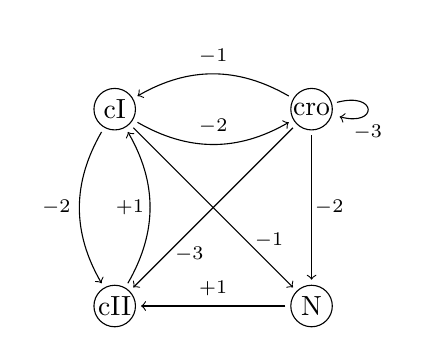
\begin{tikzpicture}[grn]
    %\path[use as bounding box] (-1.3,-0.75) rectangle (3.5,1.5);
    \node[inner sep=0] (cI) at (0,2.5) {cI};
    \node[inner sep=0] (cro) at (2.5,2.5) {cro};
    \node[inner sep=0] (cII) at (0,0) {cII};
    \node[inner sep=0] (N) at (2.5,0) {N};
    \path[->]
      (cI) edge[bend right] node[elabel, above=-4pt] {$-2$} (cro)
           edge[bend right] node[elabel, left=-2pt] {$-2$} (cII)
           edge[pos=.85] node[elabel, above=-2pt] {$-1$} (N)
      (cro) edge[bend right] node[elabel, above=-4pt] {$-1$} (cI)
            edge[loop right] node[elabel, below=-2pt] {$-3$} (cro)
            edge[pos=.65] node[elabel, below=-2pt] {$-3$} (cII)
            edge node[elabel, right=-4pt] {$-2$} (N)
      (cII) edge[bend right] node[elabel, left=-3pt] {$+1$} (cI)
      (N) edge node[elabel, above=-4pt] {$+1$} (cII);
  \end{tikzpicture}
  }
  \caption{\label{fig:phage-lambda-ig}
    Result of the IG inference performed on the PH of \todo{ref}.
  }
  \end{figure}
\end{example}

\begin{example}
  The parameters inference of \pref{pps:param_K} applied to the PH of \todo{ref}
  is conclusive for all parameters.
  The complete parametrization produced is available in \pref{tb:phage-lambda-k}.
  \begin{table}[t]
  \begin{align*}
    K_{cI, \emptyset} &= \{2\} &
    K_{cI, \{cro\}} &= \{0\} \\
    K_{cI, \{cII\}} &= \{2\} &
    K_{cI, \{cII;cro\}} &= \{2\} \\
    K_{N, \emptyset} &= \{1\} &
    K_{N, \{cro\}} &= \{0\} \\
    K_{N, \{cI\}} &= \{0\} &
    K_{N, \{cI;cro\}} &= \{0\} \\
    K_{cII, \emptyset} &= \{0\} &
    K_{cII, \{cro\}} &= \{0\} \\
    K_{cII, \{cI\}} &= \{0\} &
    K_{cII, \{cI;cro\}} &= \{0\} \\
    K_{cII, \{N\}} &= \{1\} &
    K_{cII, \{N;cro\}} &= \{0\} \\
    K_{cII, \{N;cI\}} &= \{0\} &
    K_{cII, \{N;cI;cro\}} &= \{0\} \\
    K_{cro, \emptyset} &= \{3\} &
    K_{cro, \{cro\}} &= \{2\} \\
    K_{cro, \{cI\}} &= \{0\} &
    K_{cro, \{cI;cro\}} &= \{2\}
  \end{align*}
  \caption{\label{tb:phage-lambda-k}
    Result of the parameters inference performed on the PH of \todo{ref}.
  }
  \end{table}
\end{example}




\subsection{Biological application: the epithelial growth factor receptor}\label{ssec:appli}

This subsection focuses on the study of the epidermal growth factor (EGF) receptor model detailed in~\cite{Sahin09}.
This model is represented by an IG containing 20 components and 52 edges.
A protein named EGF, having no regulator, can be considered as the only input,
and a chain of reactions leads to the activation of protein pRB which is responsible for regulating the cell division,
therefore making it essential to prevent cancer development.

Three models are created from the original IG, with different levels of precision regarding the cooperation between components.
The translation from an IG into a Process Hitting is not detailed here as it was previously covered in~\cite{PMR10-TCSB}.
Model (1) represents a translation of the raw IG into Process Hitting, that is,
without any knowledge of the Boolean rules (and therefore the cooperations) of the components.
Model (2) implements some of the rules based on the results of several knockdown experiments.
Model (3) is the totally refined model with all cooperations implemented given the Boolean functions of all components.
Therefore, those three models can be considered as successive refinements of the original and most general one.
The results of the IG and parameters inferences are detailed in \pref{tb:egfr20}
and discussed in the following alongside with details about their construction.

\begin{table}[ht]
~\hfill%\begin{center}
  \begin{tabular}{r|l|l|m{2cm}|m{2.5cm}|m{1.5cm}}
    \textbf{Model} & $\mathbf{|E|}$ & $\mathbf{|K|}$ & \textbf{Inferred parameters} & \textbf{Possible\newline models} & \textbf{Fixed points}
  \\\hline\hline
    (1) & $52$ & $196$ & $20$ & $2^{176}\simeq 9.6\cdot10^{52}$ & $0$   % v1_0.ph
  \\\hline
    (2) & $51$ & $192$ & $98$ & $2^{94}\simeq 2.0\cdot10^{28}$ & $0$    % v2_1.ph
  \\\hline
    (3) & $51$ & $192$ & $192$ & $1$ & $3$                              % ori.ph
  \\\hline
  \end{tabular}
\hfill~%\end{center}
  \caption{%
  Results of the IG and parameters inference on three models
  derived from the EGF receptor model of~\cite{Sahin09}
  with different precisions in the definition of the cooperations.
  Model (1) contains no cooperations between the components.
  Several cooperations were included in model (2) under the form of 14 cooperative sorts
  and all of them were included in Model (3) under the form of 22 cooperative sorts.
  The second column gives the number of edges in the IG inferred with \pref{pps:inference-IG}
  (the number of nodes is always the number of components in the model, that is, 20).
  The third column gives the number of parameters in the model (given the IG),
  the fourth column gives the number of parameters that could be inferred using \pref{pps:param_K},
  and the fifth column consequently gives the number of compatible models with the studied PH model,
  which exponentially depends on the number of parameters that could not be inferred.
  Finally, the last column gives the number of fixed points in the PH model,
  computed with another existing PH tool provided with \textsc{Pint}.
  }
  \label{tb:egfr20}
\end{table}

Model (1) encompasses only sole interactions between components, that is,
independent activations or inhibitions of a component on another given the regulations specified in the original IG.
Therefore, the IG inferred from model (1) is the same as the IG used to create the model,
with one additional positive auto-edge on the only input EGF (which is due to its absence of regulators).
The only parameters that could be inferred are the parameters for the extreme cases of regulation
(all activators present and all inhibitors absent, and the opposite).
This first model therefore abstracts a large number of Thomas models as a lot of parameters are left undecided.

In order to build model (2), 14 cooperative sorts were added in order to model the Boolean functions of several components
(consisting of AND and OR operands).
To do so, the following components were noticed due to their importance in the chain of reactions:
CDK4, CDK6, CycD1, ER$\alpha$ and c-MYC.
Indeed, knockdown experiments have been conducted in~\cite{Sahin09}
and the results showed that knocking down these components lead to an important decrease in the production of pRB.
We therefore concluded that these components were involved in other components' Boolean functions
in a way that the knockdown of the former was sufficient to prevent the production of the latter (which is typical of AND operands).
In order to reproduce such requirements, the Boolean functions of their successors,
that is CDK4, CDK6, prB, p21, p27, IGF1R, MYC, CycD1 and CycE1,
were modeled as cooperative sorts, if needed.
In theory, 9 cooperative sorts would have sufficed, but the chaining of cooperative sorts described
in \pref{ssec:PH} was used to reduce the number of processes in each cooperative sort.
As a result, the added cooperations allowed to infer about half the parameters;
however, the number of possible Thomas models that can be inferred from this PH is still significant
because of the numerous remaining unknown parameters.
Furthermore, we note that the inferred IG contains one edge less than the original IG. This is due to the fact that
one of the Boolean functions could in fact be simplified in a way that a component did not appear anymore in it.
No edge have therefore been inferred by our method in this case.

Finally, model (3) was build using all the Boolean functions provided in~\cite{Sahin09}.
These functions take the form of 22 cooperative sorts into the model in order to match the desired behavior of the system.
As all cooperations are fully defined in this model, all the parameters are inferred and only one Thomas model can be derived.
We note also that this PH model is the only one containing at least one fixed point.
In fact, the three found steady states include the two states that correspond to a complete propagation of the input signal,
that is, in the case where EGF is active and in the case where it is not.
The two other models contain no fixed point because some cooperations are not fully defined,
leading to oscillations that are a consequence of the nondeterministic behavior.



\subsection{Computation times on several large models}\label{ssec:cpu}

The current implementation can successfully handle large PH models of BRNs found in the literature such as:
\begin{itemize}
  \item the EGF receptor model from~\cite{Sahin09} with 20 components presented in the last
    subsection\footnote{All models mentioned in this section are available as examples distributed with \textsc{Pint}.},
  \item a T cell receptor model described as an IG in~\cite{Klamt06}, which contains 40 components and 14 cooperative sorts.
\end{itemize}
For each model, IG and parameters inferences are performed together in less than a second
on a standard desktop computer.

Bigger models related to the aforementioned systems were also tested with our implementation:
\begin{itemize}
  \item a model of the T cell receptor with 94 components, described in~\cite{SaezRodriguez2007},
  \item a model of the EGF receptor with 104 components, described in~\cite{Samaga2009}.
\end{itemize}
These two models were obtained in a previous work by an automatic translation from the CellNetAnalyzer~\cite{klamt2007structural} formalism.

The composition of all models and the results of the inferences are summarized in \pref{tb:computation}.
We note that due to a very high number of parameters, no parameters inference could be performed on the $94$ and $104$ component models.
These models would therefore be more efficiently studied as PH than as BRNs.
Finally, we note that the complexity of the method is exponential in the number of regulators of one
component and linear in the number of components.

\begin{table}[ht]
\begin{center}
  \begin{tabular}{r|c|c|c|c|c}
    \textbf{Model} & $\mathbf{|\Gamma|}$ & $\mathbf{|\PHs \setminus \Gamma|}$ & \textbf{$\Delta t$ IG} & \textbf{$\Delta t$ K} & $\mathbf{|K|}$
\\\hline\hline
    EGF receptor \cite{Sahin09} & $20$ & $22$ & <1s & <1s & 192
\\\hline
    T cell receptor \cite{Klamt06} & $40$ & $14$ & <1s & <1s & 143
\\\hline
    T cell receptor \cite{SaezRodriguez2007} & $94$ & $39$ & 100s & <1s & 578
\\\hline
    EGF receptor \cite{Samaga2009} & $104$ & $89$ & 200s & 2.5s & 27496
  \end{tabular}
\end{center}
\caption{%
  Computation times and several pieces of information related to the IG and parametrization inferences of four biological models.
  The second column gives the number of components of each model and
  the third column gives the number of cooperative sorts used to model joint actions.
  The fourth (resp.~fifth) column gives the computation times of the IG inference (resp.~the parametrization inference).
  The last column gives the number of parameters in each model.
  Due to the too high number of parameters, parametrization inference could not be performed on the $94$ and $104$ component models.
  }
\label{tb:computation}
\end{table}

\section{Conclusion and Discussion}

This work establishes the abstraction relationship between PH and Thomas' approaches for
qualitative BRN modeling.
The PH allows an abstract representation of BRNs dynamics (allowing incomplete knowledge on the
cooperation between components) that cannot be exactly represented in Ren\'e Thomas' formalism by a
single instance of BRN parametrization.
This motivates the concretization of PH models into a set of compatible Thomas' models in order to benefit
of the complementary advantages of these two formal frameworks.

We first propose an original inference of the Interaction Graph (IG) from a BRN
having its dynamics specified in the PH framework.
An IG gives a compact abstract representation of the influence of the components between each
others.
Then, based on a prior inference of Ren\'e Thomas' parametrization for BRNs from a PH model, we
delimit the set of admissible Thomas' parametrizations that are compatible with the PH dynamics,
and give arguments for their correctness.
A parametrization is compatible with the PH if its dynamics (in terms of possible transitions) is included in the PH dynamics.
The enumeration of such parametrizations is efficiently tackled using Answer Set Programming.
We illustrate the overall method with several results on large biological models.

Several extensions of the presented work are now to be considered.
First, the link between successively refined models of a system could be formally studied.
Indeed, it is convenient to refine a PH model by removing actions or adding cooperations;
the study and formalization of such process would allow to predict behavioral changes and lead to more accurate models.
Such work would also require further study on the inference of the IG in order to better understand and possibly avoid
the presence of some of the current spurious auto-edges.
Second, the inference of BRN multiplexes \cite{BernotMultiplexes} may be of practical interest 
as they allow to implicitly reduce the possible parametrizations by making cooperations appear
in the IG.
Because of its atomicity, the PH allows to specify a range of cooperations that cannot be
completely captured by a single instance of BRN multiplexes, then encouraging the inference of a set
of compatible ones.
Finally, in order to improve the performances in the IG inference, we will consider projection operations on
the PH structure to undo cooperations between components and reduce the cardinality of
configurations to explore by making the interactions independent.

\paragraph{Acknowledgement}
This work was partially supported by the Fondation Centrale Initiatives and
the French National Agency for Research (ANR-10-BLANC-0218 BioTempo project).



\bibliographystyle{elsarticle-num}
\bibliography{biblio}

%\input{parts/contributions}

\end{document}
